%% Encoding: ISO8859-1 %%

\documentclass{wissdoc}
% Autor: Roland Bless 1996-2009, bless <at> kit.edu
% Anpassungen von: Matthias Huber, Dirk Achenbach, Matthias Gabel
%                  (vorname.nachname@kit.edu)
% ----------------------------------------------------------------
% Studentische Ausarbeitung - Hauptdokument
% ----------------------------------------------------------------
% wissdoc-Optionen: draft, relaxed, pdf --> siehe wissdoc.cls
% ------------------------------------------------------------------
% Weitere packages: (Dokumentation dazu durch "latex <package>.dtx")
\usepackage{bibgerm}
\usepackage[numbers,sort&compress]{natbib}
\usepackage[protrusion=true,expansion,babel=true]{microtype}
\usepackage{amsmath}
\usepackage{txfonts}
\usepackage{dsfont}
% \usepackage{varioref}
% \usepackage{verbatim}
% \usepackage{float}    %z.B. \floatstyle{ruled}\restylefloat{figure}
% \usepackage{subfigure}
% \usepackage{fancybox} % f�r schattierte,ovale Boxen etc.
% \usepackage{tabularx} % automatische Spaltenbreite
% \usepackage{supertab} % mehrseitige Tabellen
% \usepackage[svnon,svnfoot]{svnver} % SVN Versionsinformation
%% ---------------- end of usepackages -------------

%% Informationen f�r die PDF-Datei
\hypersetup{
 pdfauthor={S�bastien Jelsch},		% TODO PDF-Informationen setzen
 pdftitle={Alternative Interpolationsverfahren}
 pdfsubject={},
 pdfkeywords={}
}

% Macros, nicht unbedingt notwendig
%% Encoding: ISO8859-1 %%

%%%%%%%%%%%%%%%%%%%%%%%
% Kommentare 
%%%%%%%%%%%%%%%%%%%%%%%
\ifnotdraftelse{
\newcommand{\Kommentar}[1]{}
}{\newcommand{\Kommentar}[1]{{\em #1}}}
% Alles innerhalb von \Hide{} oder \ignore{} 
% wird von LaTeX komplett ignoriert (wie ein Kommentar)
\newcommand{\Hide}[1]{}
\let\ignore\Hide

%%%%%%%%%%%%%%%%%%%%%%%%%
% Leere Seite ohne Seitennummer, wird aber gezaehlt
%%%%%%%%%%%%%%%%%%%%%%%%%

\newcommand{\leereseite}{% Leerseite ohne Seitennummer, n�chste Seite rechts (wenn 2-seitig)
 \clearpage{\pagestyle{empty}\cleardoublepage}
}
%%%%%%%%%%%%%%%%%%%%%%%%%%
% Flattersatz rechts und Silbentrennung, Leerraum nach rechts maximal 1cm
%%%%%%%%%%%%%%%%%%%%%%%%%%
\makeatletter
\newcommand{\myraggedright}{%
 \let\\\@centercr\@rightskip 0pt plus 1cm
 \rightskip\@rightskip
  \leftskip\z@skip
  \parindent\z@
  \spaceskip=.3333em
  \xspaceskip=.5em}
\makeatother

\makeatletter
\newcommand{\mynewline}{%
 \@centercr\@rightskip 0pt plus 1cm
}
\makeatother


%%%%%%%%%%%%%%%%%%%%%%%%%%
% F�r Index
%%%%%%%%%%%%%%%%%%%%%%%%%%
\makeatletter
\def\mydotfill{\leavevmode\xleaders\hb@xt@ .44em{\hss.\hss}\hfill\kern\z@}
\makeatother
\def\bold#1{{\bfseries #1}}
\newbox\dbox \setbox\dbox=\hbox to .4em{\hss.\hss} % dot box for leaders
\newskip\rrskipb \rrskipb=.5em plus3em % ragged right space before break
\newskip\rrskipa \rrskipa=-.17em plus -3em minus.11em % ditto, after
\newskip\rlskipa \rlskipa=0pt plus3em % ragged left space after break
\newskip\rlskipb \rlskipb=.33em plus-3em minus.11em % ragged left before break
\newskip\lskip \lskip=3.3\wd\dbox plus1fil minus.3\wd\dbox % for leaders
\newskip \lskipa \lskipa=-2.67em plus -3em minus.11em %after leaders
\mathchardef\rlpen=1000 \mathchardef\leadpen=600
\def\rrspace{\nobreak\hskip\rrskipb\penalty0\hskip\rrskipa}
\def\rlspace{\penalty\rlpen\hskip\rlskipb\vadjust{}\nobreak\hskip\rlskipa}
\let\indexbreak\rlspace
\def\raggedurl{\penalty10000 \hskip.5em plus15em \penalty0 \hskip-.17em plus-15em minus.11em}
\def\raggeditems{\nobreak\hskip\rrskipb \penalty\leadpen \hskip\rrskipa %
\vadjust{}\nobreak\leaders\copy\dbox\hskip\lskip %
\kern3em \penalty\leadpen \hskip\lskipa %
\vadjust{}\nobreak\hskip\rlskipa}
\renewcommand*\see[2]{\rlspace\emph{\seename}~#1} % from makeidx.sty

%%%%%%%%%%%%%%%%%%%%%%%%%%
% Neue Seite rechts, leere linke Seite ohne Headings
%%%%%%%%%%%%%%%%%%%%%%%%%%
\newcommand{\xcleardoublepage}
{{\pagestyle{empty}\cleardoublepage}}

%%%%%%%%%%%%%%%%%%%%%%%%%%
% Tabellenspaltentypen (benoetigt colortbl)
%%%%%%%%%%%%%%%%%%%%%%%%%%
\newcommand{\PBS}[1]{\let\temp=\\#1\let\\=\temp}
\newcolumntype{y}{>{\PBS{\raggedright\hspace{0pt}}}p{1.35cm}}
\newcolumntype{z}{>{\PBS{\raggedright\hspace{0pt}}}p{2.5cm}}
\newcolumntype{q}{>{\PBS{\raggedright\hspace{0pt}}}p{6.5cm}}
\newcolumntype{g}{>{\columncolor[gray]{0.8}}c} % Grau
\newcolumntype{G}{>{\columncolor[gray]{0.9}}c} % helleres Grau

%%%%%%%%%%%%%%%%%%%%%%%%%%
% Anf�hrungszeichen oben und unten
%%%%%%%%%%%%%%%%%%%%%%%%%%
\newcommand{\anf}[1]{"`{#1}"'}

%%%%%%%%%%%%%%%%%%%%%%%%%%
% Tiefstellen von Text
%%%%%%%%%%%%%%%%%%%%%%%%%%
% S\tl{0} setzt die 0 unter das S (ohne Mathemodus!)
% zum Hochstellen gibt es uebrigens \textsuperscript
\makeatletter
\DeclareRobustCommand*\textlowerscript[1]{%
  \@textlowerscript{\selectfont#1}}
\def\@textlowerscript#1{%
  {\m@th\ensuremath{_{\mbox{\fontsize\sf@size\z@#1}}}}}
\let\tl\textlowerscript
\let\ts\textsuperscript
\makeatother

%%%%%%%%%%%%%%%%%%%%%%%%%%
% Gau�-Klammern
%%%%%%%%%%%%%%%%%%%%%%%%%%
\newcommand{\ceil}[1]{\lceil{#1}\rceil}
\newcommand{\floor}[1]{\lfloor{#1}\rfloor}

%%%%%%%%%%%%%%%%%%%%%%%%%%
% Average Operator (analog zu min, max)
%%%%%%%%%%%%%%%%%%%%%%%%%%
\def\avg{\mathop{\mathgroup\symoperators avg}}

%%%%%%%%%%%%%%%%%%%%%%%%%%
% Wortabk�rzungen
%%%%%%%%%%%%%%%%%%%%%%%%%%
\def\zB{z.\,B.\ }
\def\dh{d.\,h.\ }
\def\ua{u.\,a.\ }
\def\su{s.\,u.\ }
\newcommand{\bzw}{bzw.\ }

%%%%%%%%%%%%%%%%%%%%%%%%%%%%%%%%%%%
% Einbinden von Graphiken
%%%%%%%%%%%%%%%%%%%%%%%%%%%%%%%%%%%
% global scaling factor
\def\gsf{0.9}
%% Graphik, 
%% 3 Argumente: Datei, Label, Unterschrift
\newcommand{\Abbildung}[3]{%
\begin{figure}[tbh] %
\centerline{\scalebox{\gsf}{\includegraphics*{#1}}} %
\caption{#3} %
\label{#2} %
\end{figure} %
}
\let\Abb\Abbildung
%% Abbps
%% Graphik, skaliert, Angabe der Position
%% 5 Argumente: Position, Breite (0 bis 1.0), Datei, Label, Unterschrift
\newcommand{\Abbildungps}[5]{%
\begin{figure}[#1]%
\begin{center}
\scalebox{\gsf}{\includegraphics*[width=#2\textwidth]{#3}}%
\caption{#5}%
\label{#4}%
\end{center}
\end{figure}%
}
\let\Abbps\Abbildungps
%% Graphik, Angabe der Position, frei w�hlbares Argument f�r includegraphics
%% 5 Argumente: Position, Optionen, Datei, Label, Unterschrift
\newcommand{\Abbildungpf}[5]{%
\begin{figure}[#1]%
\begin{center}
\scalebox{\gsf}{\includegraphics*[#2]{#3}}%
\caption{#5}%
\label{#4}%
\end{center}
\end{figure}%
}
\let\Abbpf\Abbildungpf

%%
% Anmerkung: \resizebox{x}{y}{box} skaliert die box auf Breite x und H�he y,
%            ist x oder y ein !, dann wird das uspr�ngliche 
%            Seitenverh�ltnis beibehalten.
%            \rescalebox funktioniert �hnlich, nur das dort ein Faktor
%            statt einer Dimension angegeben wird.
%%
% \Abbps{Position}{Breite in Bruchteilen der Textbreite}{Dateiname}{Label}{Bildunterschrift}
%

\newcommand{\refAbb}[1]{%
s.~Abbildung \ref{#1}}



% Print URLs not in Typewriter Font
\def\UrlFont{\rm}

\newcommand{\blankpage}{% Leerseite ohne Seitennummer, n�chste Seite rechts
 \clearpage{\pagestyle{empty}\cleardoublepage}
}

%% Einstellungen f�r das gesamte Dokument

% Trennhilfen
% Wichtig!
% Im german-paket sind zus�tzlich folgende Trennhinweise enthalten:
% "- = zus�tzliche Trennstelle
% "| = Vermeidung von Ligaturen und m�gliche Trennung (bsp: Schaf"|fell)
% "~ = Bindestrich an dem keine Trennung erlaubt ist (bsp: bergauf und "~ab)
% "= = Bindestrich bei dem Worte vor und dahinter getrennt werden d�rfen
% "" = Trennstelle ohne Erzeugung eines Trennstrichs (bsp: und/""oder)

% Trennhinweise fuer Woerter hier beschreiben
\hyphenation{
% Si-mu-la-tor
% Ab-streit-bar-keit
}

% Index-Datei �ffnen
\ifnotdraft{\makeindex}
%%%%%%%%%%%%%% includeonly %%%%%%%%%%%%%%%%%%%
% Es werden nur die Teile eingebunden, die hier
% aufgefuehrt sind!
%\includeonly{%
%titelseite,%
%erklaerung,% Ist in Kartlsruhe Pflicht (au�er f�r Studienarbeiten)
%abstract,  % Der Abstract
%einleitung,% Motivation, Zielsetzung, Gliederung
%thema,     % Das Hauptthema der Arbeit. % TODO Setze hier das eigene Thema ein!
%ergebnisse,% Ergebnisse meiner Bem�hungen
%zusammenf  % Zusammenfassung der Ergebnisse und Ausblick
%}
%%%%%%%%%%%%%%%%%%%%%%%%%%%%%%%%%%%%%%%%%%%%%%

\newcommand{\N}{\ensuremath{\mathds{N}}}		% Die nat�rlichen Zahlen
\newcommand{\Menge}[2]{\ensuremath{\{ #1 \,|\, #2 \}}}	% Darstellung parametrisierter Mengen

\begin{document}
\newgeometry{left=3cm,right=3cm,top=23mm,bottom=25mm,head=14.5pt}

\frontmatter
\pagenumbering{roman}
\ifnotdraft{
 %% Encoding: ISO8859-1 %%

%% Titelseite

\def\usesf{}
\let\usesf\sffamily % diese Zeile auskommentieren f�r normalen TeX Font

\newsavebox{\Prof}
\savebox{\Prof}{\usesf Prof.~Dr.~?.~?????????}

\begin{titlepage}
\setlength{\unitlength}{1pt}
\begin{picture}(0,0)(85,770)

\includegraphics[width=\paperwidth]{logos/KIT_Deckblatt}
\end{picture}

\thispagestyle{empty}

%\begin{titlepage}
%%\let\footnotesize\small \let\footnoterule\relax
\begin{center}
\hbox{}
\vfill
{\usesf
{\huge\bfseries Alternative Interpolationsverfahren\\		% TODO Titel der Arbeit eintragen
                im Naor-Pinkas-Broadcast-Schema \par}
\vskip 1.8cm
Studienarbeit\\	% TODO Art der Arbeit eintragen
%von\\[2mm]
\vskip 1cm

{\large\bfseries S�bastien Jelsch\\}			% TODO Namen des Autors auf dem Titelblatt eintragen
\vskip 1.2cm
Institut f�r Kryptographie und Sicherheit\\
Europ�isches Institut f�r Systemsicherheit\\
Fakult�t f�r Informatik\\
Karlsruher Institut f�r Technologie\\
%Universit�t Karlsruhe (TH)\\[2ex]
\vskip 3cm
\begin{tabular}{p{5.5cm}l}
Betreuender Professor: & {\usesf Jun.-Prof.~Dr.~D.~Hofheinz} \\	% TODO Profs eintragen
Betreuender Mitarbeiter: & Dipl.-Inf.~C.~Striecks \\	% TODO Betreuer eintragen
\end{tabular}
\vskip 3cm
Bearbeitungszeit:\qquad 15. November 2012 -- 13. Mai 2013	% TODO Bearbeitungszeit eintragen
}
\end{center}
\vfill
\end{titlepage}
%% Titelseite Ende


 \blankpage % Leerseite auf Titelr�ckseite
 %
 % Die folgende Erkl�rung ist (au�er f�r Studienarbeiten) Pflicht
 % (siehe Pr�fungsordnung)
 %% Encoding: ISO8859-1 %%

\thispagestyle{empty}
\vspace*{42\baselineskip}
\hbox to \textwidth{\hrulefill}
\par
Ich erkl�re hiermit, dass ich die vorliegende Arbeit selbst�ndig verfasst und
keine anderen als die angegebenen Quellen und Hilfsmittel verwendet habe.

Karlsruhe, den 14. Februar 2013  % TODO Datum in die Erkl�rung schreiben

%%%%%%%%%%%%%%%%%%%%%%%%%%%%%%%%%%%%%%%%%%%%%%%%%%%%%%%%%%%%%%%%%%%%%%%%
%% Hinweis:
%%
%% Diese Erkl�rung wird von der Pr�fungsordnung f�r Diplomarbeiten 
%% verlangt und ist zu unterschreiben. F�r Studienarbeiten ist diese
%% Erkl�rung nicht zwingend notwendig, schadet aber auch nicht.
%%%%%%%%%%%%%%%%%%%%%%%%%%%%%%%%%%%%%%%%%%%%%%%%%%%%%%%%%%%%%%%%%%%%%%%%
\clearpage


 \blankpage % Leerseite auf Erkl�rungsr�ckseite
}
\restoregeometry
%
%% *************** Hier geht's ab ****************
% %% Encoding: ISO8859-1 %%

\chapter*{Abstract}
\label{ch:Abstract}
%% ==============================

Lorem ipsum dolor sit amet, consectetur adipiscing elit. In tincidunt gravida est nec elementum. In vitae orci felis, convallis fringilla eros. Mauris hendrerit pulvinar augue, a laoreet erat aliquet ac. Integer suscipit lacus quis augue varius tempor. Phasellus ac quam ac dui ullamcorper fermentum. Pellentesque tellus justo, accumsan ut blandit quis, consectetur sit amet velit. Sed euismod porta metus at vestibulum. Donec quis ante ligula. Nam iaculis convallis nunc, sed cursus libero blandit eu. Praesent convallis, est sed sollicitudin fringilla, leo sapien condimentum eros, at auctor augue nunc sollicitudin sem. Aenean nibh lectus, congue vel consequat a, aliquet nec lacus.

Fusce rhoncus, metus vel accumsan dictum, libero turpis imperdiet urna, eget feugiat metus nulla at metus. Sed porttitor, leo vel luctus consectetur, est diam auctor diam, sed consequat purus velit et magna. Fusce consequat erat sit amet leo tincidunt iaculis. Curabitur nec diam non odio pharetra aliquet. Pellentesque eu odio a dui suscipit congue quis consequat elit. Duis tempus gravida magna, iaculis pellentesque orci interdum sed. Cras viverra diam in dui bibendum euismod congue nisi pellentesque. Ut a elit a ligula ultrices mattis in at leo. Nulla velit dui, porta at tincidunt sit amet, vehicula ac urna. Proin magna eros, euismod non sollicitudin id, volutpat vel ligula.

Vivamus ac egestas arcu. Duis sed felis at quam tempus venenatis sed non lectus. Integer ac posuere massa. Vivamus pulvinar velit nisi, eu consequat augue. Aenean a dolor mauris. Aenean nec eros sapien. Mauris odio dolor, suscipit nec fermentum at, facilisis ut quam. Mauris ligula neque, scelerisque non vulputate vitae, rutrum eu justo. Pellentesque in pretium massa. Phasellus quis dolor mi.


%% ++++++++++++++++++++++++++++++++++++++++++
%% Verzeichnisse
%% ++++++++++++++++++++++++++++++++++++++++++
\ifnotdraft{
{\parskip 0pt\tableofcontents} % toc bitte einzeilig
\blankpage
%\listoffigures
%\blankpage
%\listoftables
%\blankpage
}


%% ++++++++++++++++++++++++++++++++++++++++++
%% Hauptteil
%% ++++++++++++++++++++++++++++++++++++++++++
\graphicspath{{images/}}

\mainmatter
\pagenumbering{arabic}
%% Encoding: ISO8859-1 %%

\chapter{Einleitung}
\label{ch:Einleitung}

%% ==============================
\section{Motivation}
%% ==============================
\label{ch:Einleitung:sec:Motivation}
In der heutigen Welt sind Multicast-�bertragungen durch die immer weiter steigende Nachfrage nach Pay-TV, Multimedia-Anwendungen und dem zur Verf�gungstellen von gesch�tzten Inhalten zu einem sehr wichtigen und zentralen Thema geworden; denn digitale Medien sind einfach zu kopieren und zu verteilen. Dies f�hrt zu vielen n�tzlichen Programmen, gleichzeitig wird aber das illegale Kopieren von digitalen Inhalten wie Musik, Videos oder Software zu einem nicht mehr zu vernachl�ssigbarem Problem. Dies betrifft die unterschiedlichsten Formen der digitalen Verbreitung, wie beispielsweise DVDs, Satelliten- und Kabelfernsehen. Daher ist es erforderlich digitale Inhalte zu verschl�sseln, um unerlaubten Empf�ngern die M�glichkeit zu nehmen den Inhalt illegal zu verbreiten.\\
\hspace*{0.45cm}Im Gegensatz zu Punkt-zu-Punkt-Verbindungen sind die zu treffenden Sicherheitsma�nahmen bei Multicast-�bertragungen deutlich komplexer und erfordern andere Denkans�tze. Dabei handelt es sich um das folgende Problem: Wie kann ein Sender einer vordefinierten und sich st�ndig �ndernden Menge an Empf�ngern verschl�sselte Nachrichten zusenden und gleichzeitig den Inhalt vor unerlaubten Empf�ngern sch�tzen?\\
\hspace*{0.45cm}Naor und Pinkas \cite{np00} haben auf der Suche nach dieser Antwort mit Hilfe der aus der numerischen Mathematik bekannten Polynominterpolation ein Revocation-Schema entwickelt. Ein Revocation-Schema beschreibt die M�glichkeit, einer Teilmenge von Teilnehmern die Berechtigung zu entziehen, den geheimen Schl�ssel und damit verbunden die entschl�sselte Nachricht ermitteln zu k�nnen.

%% ==============================
\section{Zielsetzung}
%% ==============================
\label{ch:Einleitung:sec:Zielsetzung}
In dieser Studienarbeit wird die oben genannte Fragestellung genauer untersucht, jedoch mit dem Zusatz, andere Ans�tze zu finden. Dabei wurde im ersten Analyseschritt der Teil, der die f�r die Entschl�sselung notwendigen Informationen enth�lt, genauer betrachtet. An dieser Stelle wurde �berpr�ft, ob andere Interpolationsverfahren in diesem Schema angewendet werden k�nnen und welche Auswirkungen diese gegen�ber der von Naor und Pinkas \cite{np00} eingesetzten \mbox{Polynominterpolation} haben. Von Interesse sind dabei die notwendigen Berechnungsschritte eines Empf�ngers, die ausgef�hrt werden m�ssen, um den geheimen Schl�ssel bestimmen zu k�nnen.\\
\hspace*{0.45cm}Zudem wird die Fragestellung herangezogen, ob das Naor-Pinkas-Schema in das Asmuth-Bloom-Secret-Sharing-Schema mit eingebunden werden kann. Letzteres verwendet den aus der Zahlentheorie bekannten chinesischen Restsatz anstelle der Polynominterpolation aus der \mbox{numerischen} Mathematik.

%% ==============================
\section{Verwandte Arbeiten}
%% ==============================
\label{ch:Einleitung:sec:Verwandte-Arbeiten}
Viele hier durchgef�hrte Analysen basieren auf der von Naor und Pinkas \cite{np00} ver�ffentlichten Arbeit �ber ein Revocation-Schema mit Hilfe der Lagrange-Interpolation. In dieser Ver�ffentlichung wurden mehrere M�glichkeiten eines solchen Schemas ausf�hrlich beschrieben. Die vorliegende Studienarbeit bezieht sich jedoch ausschlie�lich auf das vorgestellte \textit{Schema f�r viele Revocations}. Zus�tzlich wurde in der vorgestellten Arbeit von Naor und Pinkas das Revocation-Schema mit einem sogenannten \textit{Self Enforcement} und \textit{Tracing} kombiniert. Letzteres wurde mit einem \textit{Black-Box-Confirmation-Test} realisiert, bei dem �berpr�ft wird, ob es sich bei einem Teilnehmer um jemanden handelt, der unerlaubt digitalen Inhalt verbreitet oder seinen pers�nlichen Schl�ssel an andere weitergegeben hat. Diese Teilnehmer werden als \textit{Traitors} bezeichnet.\\
\hspace*{0.45cm}Eine weitere verwandte Arbeit zu diesem Thema ist die Ver�ffentlichung mit dem Titel \textit{Broadcast Encryption} von Fiat und Naor \cite{fn93}. Dabei werden grundlegende Schemata vorgestellt, die dem Gruppencontroller die \mbox{M�glichkeit} geben, die verschl�sselte Nachricht an eine beliebige und sich st�ndig �ndernde Teilmenge von Empf�ngern zu versenden.\\
\hspace*{0.45cm}Das Ziel in der von Kumar et al. \cite{krs99} ver�ffentlichten Arbeit ist dem von \mbox{Naor und Pinkas} vorgestellten Revocation-Schema sehr �hnlich. Jedoch ist es mit ihrer Methode (\textit{\mbox{one-time revocation}}) m�glich, einer bestimmten Anzahl von unerlaubten Teilnehmern den Zugriff auf die geheime Information zu verwehren und gleichzeitig ist sie gegen eine vollst�ndige Vereinigung aller \mbox{Unberechtigten} sicher.

%% ==============================
\section{Gliederung}
%% ==============================
\label{ch:Einleitung:sec:Gliederung}
Der erste Abschnitt dieser Studienarbeit enth�lt eine ausf�hrliche Beschreibung der Grundlagen, wobei das Hauptaugenmerk hierbei auf dem 1979 entwickelten Secret-Sharing-Verfahren von Adi Shamir liegt.\\
\hspace*{0.45cm}Der n�chste und umfangreichste Abschnitt behandelt das von Naor und Pinkas entwickelte Revocation-Schema mit dem Versuch, dieses mit verschiedenen Polynominterpolationen erfolgreich umzusetzen. Hierbei wird die im Naor-Pinkas-Revocation-Schema verwendete Lagrange-
Interpolation detailliert beschrieben. Ferner wird versucht, die auf die Newton-Basis aufbauende Newton-Interpolation und die Spline-Interpolation erfolgreich anzuwenden und ihre Vor- und Nachteile gegen�berzustellen. Zudem wird der erforderliche Aufwand eines Teilnehmers bei den einzelnen Interpolationen ermittelt, der entsteht, um die geheime Information entschl�sseln zu k�nnen.\\
\hspace*{0.45cm}Im letzten Abschnitt wird das Asmuth-Bloom-Verfahren genauer beschrieben. Ferner wird analysiert, ob das Naor-Pinkas-Schema mit dem Asmuth-Bloom-Verfahren kombiniert werden kann.


%% Encoding: ISO8859-1 %%

\chapter{Grundlagen}
\label{ch:Grundlagen}
In dieser Studienarbeit h�ufig verwendete Begriffe werden in diesem Abschnitt genauer erl�utert. Des Weiteren werden die zugrundeliegenden Definitionen beschrieben, die in der gesamten Studienarbeit als Vorraussetzung gelten. Hierbei wird auf das von Adi Shamir entwickelte Secret-Sharing-Verfahren eingegangen, welches das Grundger�st f�r alle vorgestellten Verfahren bildet. Zus�tzlich wird das Single-Revocation-Schema von Naor und Pinkas \cite{np00} erkl�rt.

\section{Notationen und Definitionen}
\label{sec:begrifflichkeiten}

Ein \textit{Revocation-Schema} bezeichnet eine Methode um unerlaubten Teilnehmern aus einer bestimmten Teilnehmermenge die M�glichkeit zu verweigern, digitale Inhalte zu entschl�sseln. Dieser Prozess ist auch als \textit{User Exclusion} oder \textit{Blacklisting} bekannt.\\
\hspace*{0.45cm}In dieser Studienarbeit werden Revocation-Schemata vorgestellt, wobei von einem gleichbleibenden Szenario ausgegangen wird: Eine Gruppe von Teilnehmern erh�lt vom Gruppencontroller (auch als Sender oder Dealer bezeichnet) digitale Inhalte. Diese Inhalte, wie z.\,B. digitale Musik oder ein TV-Programm, werden �ber Kan�le wie das Internet, Satelliten�bertragung, Kabel oder einer DVD �bertragen. Die Informationen sind verschl�sselt und der f�r die Entschl�sselung notwendige Schl�ssel ist anf�nglich jedem Teilnehmer bekannt. Nach einer gewissen Zeit lernt der Gruppencontroller Teilnehmer kennen, die gegen die Bedingungen der Nutzungslizenz versto�en. Beispielsweise bei Nichtzahlung des Abonnements oder bei Ver�ffentlichung oder Weitergabe des geheimen Schl�ssels von einem zum anderen Teilnehmer. Dadurch ist der Gruppencontroller gezwungen diesen Traitors das Recht zu nehmen weiteren Inhalt entschl�sseln zu k�nnen.\\
\hspace*{0.45cm}Um die Effizienz eines Revocation-Schemas bestimmen zu k�nnen, m�ssen die wichtigen Faktoren der angewendeten Methoden bestimmt werden. Diese werden in drei Kategorien unterteilt:
\begin{itemize}
  \item
    \textbf{Kommunikationsaufwand}\\
    Wie viel Information muss zwischen dem Gruppencontroller und einem einzelnen Teilnehmer versendet werden, um beispielsweise den geheimen Schl�ssel zu erneuern? Hierbei wird besonders die L�nge der Nachricht untersucht.
    \newpage
  \item
    \textbf{Speicheraufwand}\\
    Wie viele und welche Informationen muss der Teilnehmer bei sich speichern, um den neuen Schl�ssel berechnen zu k�nnen? Im Allgemeinen wird hier die Anzahl an Schl�sseln betrachtet, die ein Teilnehmer f�r die Berechnung ben�tigt.
  \item
    \textbf{Berechnungsaufwand}
    \\
    Wie viele Berechnungen sind vor allem bei einem einzelnen Teilnehmer n�tig, um einen neuen Schl�ssel bestimmen zu k�nnen?
\end{itemize}
Das Verfahren von M. Naor und B. Pinkas ist deswegen interessant, da keine dieser Faktoren von der Gesamtzahl der Teilnehmer abh�ngt. Im sp�teren Verlauf wird deutlich, dass die L�nge des Schl�ssels konstant und die Kommunikation bzw. der Berechnungsaufwand linear zu der Anzahl der unerlaubten Teilnehmer ist.

F�r die Verteilung der ben�tigten Schl�ssel an die Teilnehmer wird ein Secret-Sharing-Verfahren ben�tigt. In der Kryptopgraphie bezeichnet das \textit{Secret-Sharing} eine Technik der Geheimnisteilung, wobei das Geheimnis von einem Gruppencontroller auf eine Anzahl von Instanzen aufgeteilt wird, den sogenannten \textit{Shares}. Jeder Instanz wird ein eindeutiger \textit{Share} zugewiesen und es ist nicht m�glich, ohne Zuhilfenahme zus�tzlicher Shares der weiteren Instanzen das Geheimnis zu entschl�sseln. Dieser Fall wird als einfaches Secret-Sharing-Verfahren bezeichnet. Ist jedoch nur eine gewisse Untermenge der Instanzen erforderlich um das Geheimnis zu rekonstruieren, spricht man von einem erweiterten Secret-Sharing-Verfahren oder einem $(k,n)$-Schwellenwert-Schema.\\
\hspace*{0.45cm}Es existieren mehrere M�glichkeiten, das oben genannte Schema zu konstruieren. In dieser Studienarbeit wird sich gr��tenteils auf die aus der numerischen Mathematik bekannte Polynominterpolation konzentriert.

\subsubsection{Definitionen}
\label{ch:Grundlagen:sec:Definitionen2}
Sei $\mathcal N$ die Menge aller Teilnehmer mit $n = |\mathcal N|$. Ferner existiert eine Teilmenge $\mathcal R \subset \mathcal N$ mit $t = |\mathcal R|$ Teilnehmern, die nicht das Recht und die M�glichkeit besitzen sollen, die �bertragene Nachricht zu entschl�sseln.
Ferner sei $\mathcal F$ ein endlicher K�rper und ein zuf�llig ausgew�hltes Element $\mathcal S \in \mathcal F$ der geheime Schl�ssel, welcher an die verschiedenen Teilnehmer verteilt und ausschlie�lich von den Teilnehmern $u \in \mathcal N \setminus \mathcal R$ bestimmt werden soll.


\section{Shamirs-Secret-Sharing-Schema}
\label{ch:Grundlagen:sec:Secret-Sharing-Verfahren}
Mit Hilfe des 1979 entwickelten Secret-Sharing-Verfahrens von Adi Shamir \cite{s79} ist es m�glich, ein Geheimnis auf mehrere Instanzen aufzuteilen, wobei nur eine gewisse Untermenge der Shares erforderlich ist, damit ein Teilnehmer das Geheimnis rekonstruieren kann. Dieses Schema wird auch als $(k,n)$-Schwellenwert-Schema bezeichnet, da nur $k$ der insgesamt $n$ Shares ben�tigt werden, um das Geheimnis eindeutig bestimmen zu k�nnen.\\
Hierzu erstellt der Gruppencontroller ein Polynom der Form
\[
P(x)=\mathcal S + a_1x + a_2x^2 + \dots + a_{k-1}x^{k-1}.
\]
Im n�chsten Schritt erstellt dieser zudem $n$ Wertepaare $(x_i, P(x_i))$ und verteilt diese an die Teilnehmer. Hier entspricht der Wert $x_i$ der �ffentliche und $P(x_i)$ der private Teil des Shares. Letzteres m�ssen von den Teilnehmern geheim gehalten werden.\\
Laut dem Fundamentalsatz der Algebra \cite{g15} kann ein Polynom $P$ vom Grad $k$, welches durch angegebenen $k$-St�tzwerte $P(x_i)$ verl�uft mit Hilfe von $k$ verschiedenen Wertepaaren $(x_i, P(x_i))$ eindeutig bestimmt werden. Im Vergleich zum einfachen Secret-Sharing-Verfahren eine verbesserte und effizientere Situation, da die Teilnehmer nicht alle existierenden Shares f�r die Rekonstruktion ben�tigen. Wie im Aschnitt \ref{ch:abschnitt3-2} und \ref{ch:abschnitt3-3} sp�ter gezeigt wird, existieren verschiedene M�glichkeiten und Methoden, um das Polynom eindeutig zu rekonstruieren.

\section{Single-Revocation-Schema}
\label{sec:Grundlagen:sec:Single-Revocation}
In diesem Abschnitt wird das Single-Revocation-Schema aus dem Kapitel 2.1 der Ver�ffentlichung von Naor-Pinkas \cite{np00} beschrieben. Dieses Verfahren basiert auf das Shamirs-Secret-Sharing-Schema und kann f�r einzelne Revocations (\textit{single revocations}) von bis zu $t$ Teilnehmer genutzt werden. Das Schema wird hierbei in folgende zwei Phasen gegliedert:
\begin{enumerate}
  \item
    \textbf{Vorbereitung}\\
    Gegeben sei ein K�rper $\mathcal F$. Aus diesem w�hlt der Gruppencontroller ein zuf�lliges Element $\mathcal S \in \mathcal F$, sodass dieses als Schl�ssel eines symmetrischen Verschl�sselungsschemas benutzt werden kann.
    Au�erdem generiert der Gruppencontroller in dieser Phase ein zuf�lliges, reeles Polynom $P$ vom Grad $t$ �ber $\mathcal F$ und legt mit
    \[
      \mathcal S \coloneqq P(0)
    \]
    das Geheimnis fest. Im n�chsten Schritt werden $n$ Wertepaare $I_{u_i} = (u_i, P(u_i))$ mit $i=0,\dots,n$ erstellt, wobei $\forall x_i \neq 0$ gelten muss. Anschlie�end werden diese an die jeweiligen Teilnehmer verteilt.
  \item
    \textbf{Rekonstruktion}\\
    In dieser Phase sollen die Teilnehmer $u_i \in \mathcal N \setminus \mathcal R$ das Geheimnis $\mathcal S$ ermitteln k�nnen, wobei gleichzeitig die $t$ Teilnehmer $u_{r_i} \in \mathcal R$ dies nicht k�nnen sollen.\\
    Hierzu lernt der Gruppencontroller mit der Zeit die Identit�ten der $t$ Teilnehmer $u_{r_i} \in \mathcal R$ kennen und �bermittelt folgende Nachricht an alle Teilnehmer $u_i \in \mathcal N$:
    \[
      <u_{r_1}, P(u_{r_1})>, <u_{r_2}, P(u_{r_2})>, \dots , <u_{r_t}, P(u_{r_t})>.
    \]
    Da jeder Teilnehmer sein Wertepaar $I_{u_i}$ bei sich gespeichert hat, k�nnen nach dem Fundamentalsatz der Algebra \cite{g15} ausschlie�lich die Teilnehmer $u_i \in \mathcal N \setminus \mathcal R$ den Schl�ssel $\mathcal S=P(0)$ eindeutig bestimmen, da nur diese Teilnehmer $t+1$ verschiedene St�tzstellen und St�tzwerte besitzen. Ein Teilnehmer $u_i \in \mathcal R$ besitzt mit Hilfe der �bertragenen Nachricht und der bei sich gespeicherten Information lediglich $t$ voneinander verschiedenen Wertepaare. Das Geheimnis $\mathcal S$ kann von den unerlaubten Teilnehmern nicht eindeutig bestimmt werden kann.
\end{enumerate}

\subsubsection{Nachteil des Single-Revocation-Schemas}
\label{ch:Grundlagen:sec:Broadcasting}
Aufgrund dessen, dass der geheime Schl�ssel $\mathcal S$ nach der erfolgreichen Rekonstruktion des Polynoms $P$ eindeutig bestimmbar ist, muss $\mathcal S$ bei Ver�nderung der Menge der unerlaubten Empf�nger $\mathcal R$ neu gew�hlt werden. Daher ist es notwendig, dass der Gruppencontroller ein neues, beliebiges Polynom $P$ w�hlt und jedem Teilnehmer vor der eigentlichen �bertragung des Chriffrats die pers�nlichen Shares �ber einen privaten Kanal �bermittelt. Dies ist erforderlich, da beispielsweise ein im ersten Durchlauf noch legaler Empf�nger im zweiten Durchlauf zu einem unerlaubten Empf�nger werden kann und daher nicht mehr die M�glichkeit besitzen soll, das Geheimnis bestimmen zu k�nnen. Dadurch muss in dieser Situation das Geheimnis $\mathcal S_1$ sich im zweiten Durchlauf vom Geheimnis $\mathcal S_2$ unterscheiden.


\chapter{Naor-Pinkas-Revocation-Schema}
\label{ch:np-revocation-schema}


Das in der Ver�ffentlichung von M. Naor und B. Pinkas \cite{np00} vorgestellte Verfahren stellt eine abstrakte Definition eines Revocation-Schemas dar. Die Hauptaufgabe des Verfahrens bezieht sich darauf, auf geschickte Art und Weise eine Verteilung des geheimen Schl�ssels sicherzustellen, sodass aus einer beliebig gro�en Menge von erlaubten Empf�ngern bis zu maximal $t$ Empf�nger ausgeschlossen werden k�nnen.

In der vorgestellten Arbeit werden drei Schemata vorgestellt um unerlaubten Teilnehmern den Zugriff auf den Schl�ssel und somit auf den Inhalt zu verweigern. Dabei konzentriert sich diese Studienarbeit ausschlie�lich auf das zweite vorgestellte Schema aus Kapitel 2.2 in \cite{np00}.

%% ==============================
\section{Verfahren}
\label{ch:np-revocation-schema:sec:Verfahren}
%% ==============================

Das nun vorgestellte Schema ist f�r eine Anzahl von maximal $t$ zu sperrende Empf�nger sicher und basiert auf der Decisional-Diffie-Hellman-Annahme.

\subsection{Decisional-Diffie-Hellman-Annahme}
% Die Decisional-Diffie-Hellman-Annahme (DDH) wird f�r die Konstruktion effizienter kryptographischer Funktionen genutzt, die eine sehr starke Sicherheit garantieren sollen. Diese enth�lt das Diffie-Hellman-Schl�sselvereinbarungsprotokoll \cite{dh79}, das ElGamal-Verschl�sselungsschema \cite{e85}, pseudozuf�llige Funktionen \cite{nr97} und eine Konstruktion eines Kryptosystems, welches gegen Choosen-Ciphertext-Angriffe \cite{cs98} sicher ist.\\
% \hspace*{0.45cm}
Gegeben sei eine endliche und zyklische Gruppe $\mathcal G$ mit einem Erzeuger $g$. Das bedeutet, dass zu jedem Element $f$ der Gruppe $\mathcal G$ eine Ganzzahl $z$ mit $f = g^z$ existiert. Bei der DDH-Annahme geht es darum, dass kein effizienter Algorithmus existiert, der zwischen den Verteilungen $<g^a, g^b, g^{ab}>$ und $<g^a, g^b, g^c>$ mit zuf�lligen und beliebigen $a,b,c$ aus $[1,\dots,|\mathcal G|]$ unterscheiden kann. Anders gesagt, kann unter der DDH-Annahme kein Angreifer den Wert $g^{ab}$ von einem zuf�lligen Gruppenelement unterscheiden.

\subsection{Schema f�r viele Revocations}
Das vorgestellte Schema aus Kapitel 2.2 der Ver�ffentlichung von Naor und Pinkas \cite{np00} ist �ber eine Untergruppe $\mathbb Z_q$ mit Ordnung $q$ in $\mathbb Z_p^*$ definiert, wobei $p$ eine Primzahl und $q|p-1$ definiert ist. Au�erdem sei ein Erzeuger $g$ aus $\mathbb Z_q$ gegeben, sodass die Decisional Diffie-Hellman Annahme f�r $\mathbb Z_q$ und $g$ zutrifft.\\
% Dieses Schema verwendet die zuvor ver�ffentlichte Idee von Feldman \cite{f87}, in der der erste Versuch beschrieben wurde, Shamirs-Secret-Sharing-Verfahren in den Exponenten zu verlagern.
\hspace*{0.45cm}Dieses Schema kann f�r viele Revocations genutzt werden, solange verhindert wird, dass mehr als $t$ Teilnehmer ausgeschlossen werden sollen. Zudem wird sp�ter gezeigt, dass das Verfahren bis auf eine Vereinigung von $t$ unerlaubte Teilnehmer sicher ist.\\
\hspace*{0.45cm}Um das Schema umzusetzen, werden folgende zwei Phase ben�tigt:
\begin{itemize}
  \item
    \textbf{Initialisierungsphase}\\
    In dieser Phase generiert der Gruppencontroller ein beliebiges Polynom $P$ vom Grad $t$ welches �ber die Gruppe $\mathbb Z_q$ definiert ist. Nach diesem Schritt ver�ffentlicht der Gruppencontroller �ber einen privaten Kanal $p$ und $q$ und sendet jedem Teilnehmer $u$ seinen eindeutigen und pers�nlichen Schl�ssel
    \[
      \mathcal K_u=<I_u, P(I_u)>.
    \]
    Dabei entspricht der Wert $I_u$ der �ffentliche Teil des Shares und beschreibt gleichzeitig das zum Teilnehmer $u$ geh�rende Identifizierungsmerkmal. Wichtig zu betonen ist, dass diese Phase ein einziges Mal f�r alle sp�ter folgenden Revocations durchgef�hrt werden muss.
  \item
    \textbf{Revocation-Phase}\\
    In dieser Phase wird den unerlaubten Teilnehmern die M�glichkeit genommen, die vom Gruppencontroller �bermittelte Nachricht zu ermitteln.\\
    Dabei m�ssen die Identit�ten der $t$ Teilnehmer $\mathcal R=\lbrace I_{u_1}, \dots, I_{u_t}\rbrace$ herausgefunden werden, die aus der Menge der erlaubten Empf�nger ausgeschlossen werden sollen. Da dies nicht Teil des Revocation-Schemas ist, wird dieser Prozess hier nicht n�her erl�utert. In der Ver�ffentlichung \cite{np00} kann das Verfahren im Kapitel 3.4 betrachtet werden.\\
    Ist die unerlaubte Teilnehmermenge $\mathcal R$ bekannt, w�hlt der Gruppencontroller ein zuf�lliges, beliebiges $r \in \mathbb Z_q$ und setzt
    \[
      \mathcal S=g^{rP(0)}
    \] als neuen Schl�ssel fest. Zudem werden f�r alle Empf�nger $I_{t_i} \in \mathcal R$ der Wert $g^{rP(I_{t_i})}$ berechnet. Im n�chsten Schritt �bermittelt der Gruppencontroller jedem Empf�nger $u \in \mathcal N$ die berechneten Werte und den pers�nlichen Schl�ssel der unerlaubten Empf�ngern:
    \[
    <g^r, g^{rP(I_{u_1})}, g^{rP(I_{u_2})}, \dots ,g^{rP(I_{u_t})}, I_{u_1},  I_{u_2}, \dots,  I_{u_t} >
    \]
\end{itemize}

Jeder Empf�nger $u \in \mathcal N \setminus \mathcal R$ besitzt mit der bei sich gespeicherten Information $\mathcal K_u=<I_u, P(I_u)>$ die notwendige ($t+1$)-te Information um das Polynom $P$ vom Grad $t$ eindeutig bestimmen zu k�nnen. Der Empf�nger $u$ berechnet $(g^r)^{P(I_u)}$ und besitzt aufgrund dessen ($t+1$) St�tzstellen $I_u, I_{u_1}, \dots I_{u_t}$ und die dazugeh�renden ($t+1$) St�tzwerte $(g^r)^{P(I_u)},(g^r)^{P(I_{u_1})},\dots,(g^r)^{P(I_{u_t})}$. Mit Hilfe einer beliebigen Polynominterpolation wird das Interpolationspolynom eindeutig rekonsturiert. Der letzte Schritt beim Empf�nger besteht aus der Berechnung von $(g^r)^{P(0)}$, um den Schl�ssel $\mathcal S$ zu erhalten.\\
\hspace*{0.45cm}Ein Empf�nger $u_{t_i} \in \mathcal R$ besitzt w�hrenddessen mit Hilfe der �bertragenen Nachricht und der gespeicherten Information $\mathcal K_{u_i} = <I_{u_i}, P(I_{u_i})>$ nur insgesamt $t$ verschiedene St�tzwerte und St�tzstellen. Zu wenig um das Interpolationspolynom vom Grad $t$ durch die angegebenen St�tzstellen eindeutig bestimmen zu k�nnen.

\subsection{Unerlaubte Empf�ngermenge $\mathcal R$}
Sollte zu einem beliebigen Zeitpunkt $t' < t$ unerlaubte Empf�nger existieren, fehlen auch jedem erlaubten Teilnehmer ($t-t'$) St�tzstellen um mit Hilfe einer Polynominterpolation das Interpolationspolynom vom Grad $t$ zu bestimmen. Dieses Problem kann durch den Gruppencontroller behoben werden:\\
\hspace*{0.45cm}Existieren zu einem beliebigen Zeitpunkt $t' < t$ unerlaubte Empf�nger, erstellt der Gruppencontroller ($t-t'$) Dummy-Benutzer aus $P$, wobei diese Dummy-Benutzer von allen existierenden Teilnehmern verschieden sein m�ssen. Diese werden mit den realen unerlaubten Teilnehmer an alle $u \in \mathcal N$ versendet, sodass zu jedem Zeitpunkt sichergestellt wird, dass $t$ St�tzstellen �bermittelt werden.

\subsection{Mehrfachausf�hrung}
\label{ch:np-revocation-schema:sec:multi}
Im Abschnitt \ref{sec:Grundlagen:sec:Single-Revocation} wurde beim Single-Revocation-Schema das Problem der Mehrfachausf�hrung erkl�rt. Hierbei muss der Gruppencontroller bei Ver�nderung der Menge $\mathcal R$ ein neues Polynom $P$ und somit einen neuen Schl�ssel $\mathcal S$ bestimmen. Dadurch ist es erforderlich, dass jeder Teilnehmer $u_i$ eine neue pers�nliche Information $\mathcal K_{u_i} = <I_{u_i}, P(I_{u_i})>$ zugewiesen bekommt.\\
\hspace*{0.45cm}Diese Schritte sind beim Schema f�r viele Revocations nicht notwendig. Gegeben sei die Menge $\mathcal R=\lbrace I_{u_1},\dots,I_{u_{t-1}}, I_{u_{d}} \rbrace$ mit einem Dummy-Benutzer $I_{u_d}$. Sollte ein bei der ersten �bertragung erlaubter Teilnehmer $u_j$ bei der zweiten �bertragung nicht mehr das Recht besitzen den Schl�ssel $\mathcal S$ zu bestimmen, wird der Dummy-Benutzer aus der Menge $\mathcal R$ entfernt und durch den Teilnehmer $I_{u_j}$ ersetzt. Die Menge sieht demnach wie folgt aus: $\mathcal R=\lbrace I_{u_1},\dots,I_{u_{t-1}}, I_{u_{j}} \rbrace$. In der Revocation-Phase w�hlt der Gruppencontroller ein beliebiges $r^\prime \in \mathbb Z_q$ und erh�lt somit einen neuen Schl�ssel $\mathcal S^{\prime}$. Die �bertragene Nachricht sieht daraufhin wie folgt aus:
\[
  <g^{r^\prime}, g^{r^\prime P(I_{u_1})}, g^{r^\prime P(I_{u_2})}, \dots ,g^{r^\prime P(I_{u_{t-1}})}, g^{r^\prime P(I_{u_{d}})} , I_{u_1},  I_{u_2}, \dots,  I_{u_{t-1}}, I_{u_d} >
\]
Jeder Teilnehmer $u_i\in \mathcal N \setminus \mathcal R$ besitzt mit seiner pers�nlichen Information $\mathcal K_{u_i} = <I_{u_i}, P(I_{u_i})>$ und der Berechnung von $(g^r)^{P(I_{u_i})}$ weiterhin ($t+1$) verschiedene St�tzwerte und St�tzstellen. Das Polynom kann eindeutig an der Stelle $\mathcal S^\prime = g^{r^\prime P(0)}$ bestimmt werden.\\
\hspace*{0.45cm}Der Gruppencontroller muss zu keinem Zeitpunkt ein neues Polynom bestimmen, da der Wert $P(0)$ durch die Zuhilfenahme des Erzeugers $g$ aus $\mathbb Z_q$ keinem Teilnehmer bekannt ist.

\subsection{Empf�nger hinzuf�gen}
\label{ch:np-revocation-schema:sec:add-user}
Der Gruppencontroller kann jederzeit neue Empf�nger hinzuf�gen, auch wenn diese nach der Initialisierungsphase hinzukommen. Sei $u_{new}$ der neue Empf�nger. Der Gruppencontroller weist ihm eine neue, eindeutige und noch nicht verwendete Identit�t $I_{u_{new}}$ zu und sendet das ihm zugeordnete Wertepaar $\mathcal K_{u_{new}}= <I_{u_{new}},P(I_{u_{new}})>$ �ber einen privaten Kanal mit. Bei der n�chsten �bertragung kann der Benutzer bereits $\mathcal S = g^{rP(0)}$ mit Hilfe der �bermittelten $t$ St�tzstellen und -werte berechnen.

\subsection{Empf�nger aus $\mathcal R$ entfernen}
Gegeben sei ein Empf�nger $u_l$ der bei der letzten �bertragenen Nachricht zum Zeitpunkt $t_{-1}$ den Schl�ssel $\mathcal S$ nicht bestimmen durfte, ihm jedoch beim darauffolgenden Zeitpunkt $t_{0}$ dieses Recht erneut gegeben wurde. Anders ausgedr�ckt, war der Empf�nger zum Zeitpunkt $t_{-1}$ $u_l \in \mathcal R$ und zum Zeitpunkt $t_{0}$ $u_l \in \mathcal N \setminus \mathcal R$. In diesem Szenario reicht es aus, dass der Gruppencontroller den Empf�nger $u_l$ aus der �bertragenen Nachricht als unerlaubten Empf�nger entfernt und durch einen Dummy-Benutzer oder einen anderen, unerlaubten Empf�nger ersetzt. Der Empf�nger ben�tigt keinen neuen pers�nlichen Schl�ssel $\mathcal K_{u_l}$ und der Gruppencontroller braucht keinen neuen Schl�ssel $\mathcal S$ oder ein Polynom $P$ zu bestimmen. Denn die ihm zugewiesene pers�nliche Information $P(u_l)$ ist lediglich dem Gruppencontroller und dem Teilnehmer $u_l$ bekannt. Durch das Verlagern der Information in den Exponenten mit Hilfe des Erzeugers $g$ und dem vor jeder �bertragung zuf�llig ausgew�hlten $r$ bleibt $P(u_l)$ aufgrund der Berechnung $g^{rP(u_l)}$ den anderen Empf�ngern unbekannt.

\subsection{Speicheraufwand}
Jeder Teilnehmer $u$ muss seine pers�nliche Information $\mathcal K_u$ speichern. Das sind in diesem Fall ein Element $I_u \in \mathbb Z_q$ und der dazugeh�rige Wert des $P(I_u) \in \mathbb R$. F�r den geheimen Schl�ssel muss jeder Empf�nger lediglich ein weiteres Element aus $\mathbb Z_q$ speichern.\\
\hspace*{0.45cm}Die Revocation-Nachricht hat eine L�nge von $O(t)$. Genauer gesagt enth�lt die Nachricht ($t+1$) Elemente aus $Z^*_p$ und $t$ Elemente aus $Z_q$.\\
\hspace*{0.45cm}Der Gruppencontroller muss, im Gegensatz zu einem Teilnehmer, etwas mehr Speicherkapazit�t aufweisen. Dieser speichert das generierte Polynom $P$ und alle vergebenen St�tzstellen, um eine doppelte Zuweisung zweier Teilnehmer zu vermeiden. Zudem m�ssen alle unerlaubten Empf�nger markiert werden, um diese in der Nachricht �bermitteln zu k�nnen.

\subsection{Sicherheit}
Im Abschnitt \ref{ch:np-revocation-schema:sec:multi} wurde gezeigt, dass das Verfahren von Naor und Pinkas wiederholt f�r Revocations angewendet werden kann. Das Verfahren ist auch sicher wenn $t$ Teilnehmer sich zusammenschlie�en. Solch ein Zusammenschluss von Benutzern kann unter der DDH-Annahme zu keinem Zeitpunkt zwischen dem Gruppenschl�ssel und einem zuf�lligen Wert unterscheiden.\\
\hspace*{0.45cm}Die ausf�hrliche Beweisidee der letzten Aussage kann in der Ver�ffentlichung von Naor und Pinkas \cite{np00} nachgelesen werden.

% \begin{proof}[\textbf{Beweisidee aus \cite{np00}}]
% \hspace*{0.45cm}Der Beweis basiert auf die DDH-Annahme. Aus Gr�nden der �bersichtlichkeit wird der Beweis zun�chst f�r den Fall $t=1$ gezeigt.\\
% \hspace*{0.45cm}Angenommen das Verfahren sei f�r $t=1$ unsicher und kann von einem Teilnehmer $v$ gebrochen werden. Dieser f�hrt einen Algorithmus $D'$ aus, der folgende Eingabe erh�lt: den Wert $P(I_v)$ des linearen Polynoms $P$ und polynomiell viele generierte Tupel $<g^{r_i}, g^{r_iP(I_v)}, g^{r_iP(0)}>$ mit zuf�llig ausgew�hltem $r_i$ und den dem Teilnehmer $v$ bekannten Informationen $g^r$ und $g^{rP(I_v)}$. Diese Tupel wurden ihm w�hrend der Revocation-Phase bekannt, in welcher er ein legaler Teilnehmer war. Wenn die Annahme stimmt, kann $D'$ zwischen $g^{rP(0)}$ und einem zuf�lligen Wert unterscheiden.\\
% \hspace*{0.45cm}Hierf�r wird ein Algorithmus $D$ konstruiert, welcher $D'$ nutzt, um die DDH-Annahme zu brechen. Die Eingaben von $D$ sind $g^a$, $g^b$ und ein Wert $C$, welcher entweder $g^{ab}$ oder ein zuf�lliger Wert ist. $D$ erstellt die Eingaben f�r $D'$, wobei $P(0)=b$ und $r=a$ als geplantes Ziel gesetzt werden. Zudem generiert der Algorithmus $D$ einen zuf�lligen Schl�ssel $<I_v, P(I_v)>$ und �bergibt diesen an $D'$. Im n�chsten Schritt werden mit zuf�lligen Werten $r_i$ viele verschiedene Tupel der Form $<g^{r_i}, g^{r_iP(I_v)}, g^{r_ib}>$ erstellt und an $D'$ �bergeben. Als n�chstes werden $D'$ die weiteren Werte $(g^a, g^{aP(I_v)}, C)$ von $D$ �bertragen. Letzterer gibt die gleiche Antwort wie der Algorithmus $D'$ aus. Dabei handelt es sich um die Ausgabe, ob es sich beim Wert $C$ um $g^{ab}$ handelt oder nicht. Die Erfolgswahrscheinlichkeit von $D'$ im Brechen der DDH-Annahme ist die gleiche Wahrscheinlichkeit wie die, dass $D'$ das Revocation-Schema bricht.\\
% \hspace*{0.45cm}Nun wird die Situation einer Vereinigung von $t$ korrupten Teilnehmern $1,\dots,t$ genauer betrachtet. Diese f�hren einen Algorithmus $D'$ aus, welcher folgende Eingaben erh�lt: Die Werte $P(I_1),\dots,P(I_t)$ des linearen Polynoms $P$ mit den St�tzwerten $I_1,\dots,I_t$, polynomiell viele Tupel $<g^{r_i},g^{r_iP(I_1)},\dots,g^{r_iP(I_t)}>$ generiert mit zuf�llig ausgew�hlten $r_i$. Diese Werte werden der Vereinigung der korrupten Teilnehmer anhand der Revocation-Nachricht bekannt, wenn mindestens ein Teilnehmer nicht in der Menge $\mathcal R$ vorkam. Zudem wird dem Algorithmus $D'$ ein Tupel der Form $g^r, g^{rP(I_1)}, \dots, g^{rP(I_t)}$ �bergeben, d.\,h. f�r jeden bekannten Wert $P(I_u)$ in der Vereinigung existiert ein dazugeh�riger Wert $g^{rP(I_u)}$ im Tupel. Wenn die Annahme korrekt ist, kann $D'$ mit Hilfe dieser Informationen zwischen $g^{rP(0)}$ und einem zuf�lligen Wert unterscheiden.\\
% \hspace*{0.45cm}Unter Anwendung von $D'$ k�nnen wir erneut einen Algorithmus $D$ konstruieren, welcher die DDH-Annahme bricht. Die Eingaben von $D$ sind $g^a,g^b$ und ein Wert $C$, welcher entweder $g^{ab}$ oder ein Zufallswert ist. Im n�chsten Schritt generiert $D$ die Eingaben f�r $D'$. Dieser erzeugt daraufhin zuf�llige Schl�ssel der Form $\lbrace<I_j,P(I_j)>\rbrace_{j=1}^{\,t}$ und �bergibt diese an $D'$. Anschlie�end generiert $D$ mit zuf�lligen Werten $r_i$ die Tupel $<g^{r_i}, g^{r_iP(I_1)}, \dots, g^{r_iP(I_t)}>$ und �bergibt auch diese $D'$. \mbox{Daraufhin} �bertr�gt $D$ die Werte $(g^a, g^{aP(I_1)}, \dots, g^{aP(I_t)}, C)$ an $D'$ und gibt dieselbe Antwort wie der Algorithmus $D'$ zur�ck (ob es sich beim Wert $C$ um $g^{ab}$ handelt oder nicht). Auch hier ist die Erfolgswahrscheinlichkeit von $D'$, dass dieser die DDH-Annahme bricht, genauso hoch wie die des Brechens des Revocation-Schemas.\newline
% \end{proof}
% $\qedhere$\\

\newpage


\section{Naor-Pinkas-Polynom-Interpolation mit Lagrange}
\label{ch:abschnitt3-2}
Im vorherigen Abschnitt \ref{ch:np-revocation-schema:sec:Verfahren} wurde das von M. Naor und B. Pinkas entwickelte Verfahren vorgestellt, jedoch ohne Angabe eines konkreten Interpolationsverfahrens f�r das Polynom $P$. Die in der ver�ffentlichten Arbeit von Naor und Pinkas \cite{np00} angewendete Lagrange-Interpolation wird in diesem Abschnitt das Hauptthema sein.

%% ==============================
\subsection{Lagrange-Interpolationsaufgabe f�r Polynome}
\label{ch:np-revocation-schema:sec:Mathematische Definition}
%% ==============================
Mit Hilfe der Lagrange-Interpolation wird in der numerischen Mathematik nach einem eindeutigen Polynom gesucht, welches exakt durch angegebene, paarweise verschiedene Punkte verl�uft.

Dabei seien ($t+1$) paarweise verschiedene St�tzstellen $x_i \in \mathbb R$ mit $i=0,\dots,t$ und die zugeh�rigen Werte $y_i$, die sogenannten St�tzwerte, bekannt. Das Problem bei der Interpolation lautet wie folgt: Gesucht wird nach einem reelen Polynom $P$ von H�chstgrad $t$, welches alle Gleichungen $P(x_i)=y_i$ erf�llt. Dabei bezeichnet man die Polynome
\begin{align*}
\lambda_{i}(x) \coloneqq \prod_{j=0,\,j \neq i}^t \frac{x-x_j}{x_i-x_j}
\end{align*}
als die zur St�tzstelle $x_i$ geh�renden Lagrange-Grundpolynome. Das Interpolationsproblem l�sst sich in der Lagrange-Form mit Hilfe der $\lambda_i$ direkt darstellen:
\begin{align*}
P(x) \coloneqq \sum_{i=0}^t \lambda_i(x) \cdot y_i
\end{align*}
Nach dem Fundamentalsatz der Algebra \cite{g15} existiert ein solches Polynom stets und ist eindeutig bestimmbar. Das Polynom wird als Lagrange'sches Interpolationspolynom in der Langrange'schen Darstellung bezeichnet. Die eben aufgef�hrte Formel unterstreicht zudem, dass eine lineare Abh�ngigkeit zwischen $P$ und den St�tzstellen $y_i$ besteht. Wie sp�ter gezeigt wird, kann diese Eigenschaft in gewissen Situationen von Vorteil sein.

%% ==============================
\subsection{Lagrange-Interpolation im Naor-Pinkas-Verfahren}
%% ==============================
\label{ch:np-revocation-schema:sec:Lagrange}
Der Gruppencontroller generiert ein zuf�lliges Polynom $P$ vom Grad $t$ �ber $\mathbb Z_q$ und erstellt f�r jeden Empf�nger $u$ ein pers�nliches Wertepaar $K_{u_0} = <I_{u_0}, P(I_{u_0})>$. Dieses wird �ber einen privaten Kanal an den Empf�nger $u_0$ gesendet, wobei $I_{u_0}$ ein nichtgeheimes Indentifizierungsmerkmal beschreibt. Zudem w�hlt der Gruppencontroller ein zuf�lliges $r \in \mathbb Z_q$ und setzt $g^{rP(0)}$ als neuen Schl�ssel $\mathcal S$ fest. Nach diesen Schritten �bermittelt der Gruppencontroller folgende Nachricht alle Empf�nger $u\in \mathcal N$:
\begin{align*}
<g^r, g^{rP(I_{u_1})}, g^{rP(I_{u_2})}, \dots ,g^{rP(I_{u_t})}, I_{u_1},  I_{u_2}, \dots,  I_{u_t}>
\end{align*}
Mit Hilfe der Lagrange-Interpolation soll jeder Empf�nger $u \in \mathcal N\setminus \mathcal R$ das vom Gruppencontroller generierte Polynom eindeutig bestimmen k�nnen. Zu Beginn berechnet $u$ den Wert $(g^r)^{P(I_{u_0})}$ und wertet das erste Lagrange-Grundpolynom
\begin{align*}
\lambda_0 \coloneqq \lambda_0(0) = \prod_{j=1}^t \frac{-I_{u_j}}{I_{u_0}-I_{u_j}} = \prod_{j=1}^t \frac{I_{u_j}}{I_{u_j}-I_{u_0}}
\end{align*}
an der gew�nschten Stelle $x=0$ aus.\\
\newpage
Die beiden Werte kann lediglich der Empf�nger $u_0$ berechnen, da das Wertepaar $K_{u_0} = <I_{u_0}, P(I_{u_0})>$ nur ihm bekannt ist.
Im n�chsten Schritt werden mit Hilfe der �bermittelten Nachricht die weiteren erforderlichen $t$ Lagrange-Grundpolynome berechnet:
\begin{align*}
\lambda_i = \prod_{j=0,j\neq i}^t \frac{I_{u_j}}{I_{u_j}-I_{u_i}}
\end{align*}
Die Berechnung des Schl�ssels $\mathcal S$ erfolgt nach folgenden Berechnungsschritten:
\begin{align*}
\mathcal S & = (g^r)^{P(0)}\\
& = (g^r)^{\sum_{i=0}^t \lambda_i P(I_{u_i})}\\
& = \prod_{i=0}^t (g^r)^{\lambda_i P(I_{u_i})}\\
& = \prod_{i=0}^t (g^{r P(I_{u_i})})^{\lambda_i}
\end{align*}
Mit Hilfe des vom Gruppencontroller �bertragenen Wertes $g^r$ und der pers�nlichen Information $K_{u_0} = <I_{u_0}, P(I_{u_0})>$ kann jeder Empf�nger $u \in \mathcal N \setminus \mathcal R$ das Polynom eindeutig an der Stelle $g^{rP(0)}$ bestimmen, da nur diese die erforderlichen ($t+1$) Wertepaare $<(I_{u_i}, P(I_{u_i})>$ mit $i=0,\dots,t$ besitzen. Einem Empf�nger $u_r \in R$ fehlt das notwendige ($t+1$)-te Wertepaar, da seine St�tzstelle bereits in der �bermittelten Nachricht vorkommt und somit doppelt vorhanden ist.

\subsection{Aufwand}
\label{ch:np-revocation-schema:sec:Aufwand}
Um den Rechenaufwand der Lagrange-Interpolation im Naor-Pinkas-Verfahren ermitteln zu k�nnen, werden die jeweiligen Berechnungsschritte eines Empf�ngers genauer betrachtet. Die Formel f�r die Berechnung eines einzelnen Lagrange-Grundpolynoms lautet:
\begin{align*}
  \lambda_i &= \prod_{j=0,\,j\neq i}^t \frac{I_{u_j}}{I_{u_j}-I_{u_i}}
  = \frac{
    I_{u_0} \cdot \ldots \cdot I_{u_{i-1}} \cdot I_{u_{i+1}} \cdot \ldots \cdot I_{u_t}
  }{
    (I_{u_0}-I_{u_i})\cdot \ldots \cdot (I_{u_{i-1}}-I_{u_i}) \cdot (I_{u_{i+1}}-I_{u_i})\cdot \ldots \cdot (I_{u_t}-I_{u_i})
  }
\end{align*}
Dabei werden im Z�hler insgesamt ($t-1$) Mutliplikationen (M) und im Nenner ($t-1$) M und $t$ Additionen (A) ben�tigt. Zudem kommt zum Schluss eine Division (D) dazu. Zusammengefasst ergibt das f�r ein einzelnes Lagrange-Grundpolynome folgenden Aufwand:
\[
  2\cdot (t+1)\,M + 1\, D  + t\, A.
\]
Die Berechnung muss f�r jede der ($t+1$) St�tzstellen ausgef�hrt werden. Der Rechenaufwand f�r alle Lagrange-Grundpolynome steigt dadurch auf insgesamt
\begin{align}
\label{eq:la_auf_grundpol}
&\hspace*{0.45cm} (t+1)\cdot ( 2\cdot(t+1)\,M +1\,D + t\,A )\notag\\
&= 2\cdot (t+1)^2\,M + (t+1)\,D + t\cdot(t+1)\,A
\end{align}
an. Die n�chsten Berechnungen erfolgen bei der Ermittlung des geheimen Schl�ssels $\mathcal S$. Mit Hilfe des vom Gruppencontroller �bertragenen Wertes $g^r$ kann der Empf�nger $(g^r)^{P(I_{u_0})}$ berechnen. Offensichtlich kostet dies eine Exponentenberechnung (E). Um das Polynom letztendlich an der Stelle $P(0)$ ermitteln zu k�nnen, muss die folgende Formel ausgef�hrt werden:
\[
\prod_{i=0}^t (g^{r P(I_{u_i})})^{\lambda_i}=(g^{r P(I_{u_0})})^{\lambda_0} \cdot \ldots \cdot (g^{r P(I_{u_t})})^{\lambda_t}
\]
Zum einen sind dank der �bertragenen Nachricht die Werte in den Klammern bekannt, zum anderen m�ssen die Exponenten noch berechnet werden. Dies erh�ht den Aufwand auf weitere ($t+1$) E. Der Berechnungsaufwand betr�gt demnach
\begin{align}
\label{eq:la_auf_formel}
t\,M + (t+2)\,E .
\end{align}


Nach den Ergebnissen aus \eqref{eq:la_auf_grundpol} und \eqref{eq:la_auf_formel} betr�gt der Gesamtaufwand f�r einen Empf�nger mit der Lagrange-Interpolation im Naor-Pinkas-Verfahren
\begin{align}
\label{eq:la_formel_gesamt}
&\hspace*{0.45cm} 2\cdot (t+1)^2\,M + (t+1)\,D + t\cdot(t+1)\,A + t\,M + (t+2)\,E \notag\\
&= \left(2\cdot (t+1)^2+t\right)\,M+(t+1)\,D + t\cdot(t+1)\,A + (t+2)\,E.
\end{align}

\subsection{Fazit}
\label{ch:np-revocation-schema:sec:Fazit}
Die Lagrange-Interpolation wird in der Praxis eher selten angewendet. Zum einen ist bei einer gro�en Anzahl von St�tzstellen der Rechenaufwand verh�ltnism��ig gro�, da f�r alle ($t+1$) St�tzstellen jeweils ein Lagrange-Grundpolynom berechnet werden muss, was zum Gesamtaufwand wie in \eqref{eq:la_formel_gesamt} dargestellt f�hrt. Zum anderen ist bei Hinzunahme lediglich einer einzelnen St�tzstelle eine Neuberechnung aller $\lambda_i$ notwendig.\\
\hspace*{0.45cm}Ein Vorteil der Lagrange-Darstellung ist jedoch, dass sich die Summen aus den aus Produkten bestehenden Br�chen besonders einfach in Form von ineinander geschachtelten Schleifen programmieren und somit einfacher in Programmen einbeziehen lassen. Zudem werden die St�tzwerte unabh�ngig von den St�tzstellen berechnet. Sobald die Lagrange-Grundpolynome $\lambda_i$ bestimmt wurden, lassen sich verschiedene S�tze von St�tzwerten $y_i$ mit gleichen St�tzstellen $x_i$ schneller interpolieren. Auf das Verfahren von M. Naor und B. Pinkas bezogen ein enormer Vorteil, da in einem Zeitraum bei Nichtver�nderung der unerlaubten Empf�ngermenge die weiteren Empf�nger $u \notin R$ durch lokale Speicherung der Lagrange-Grundpolynome $\lambda_i$ nicht mehr neu berechnet werden m�ssen. Aufgrund dieser Eigenschaft l�sst sich nach einmaliger Berechnung der $\lambda_i$ und in einem Zeitraum ohne �nderung der Menge $\mathcal R$ der Rechenaufwand auf $t$ Multiplikationen und $(t+2)$ Exponentenberechnungen reduzieren. Zudem kann in diesem speziellen Zeitraum auch die zu �bertragende Nachrichtenl�nge um die Menge der zu sperrenden Empf�nger $\mathcal R = \{I_{u_1},\dots,I_{u_t}\}$ verk�rzt werden, da diese wegen den bereits berechneten und lokal gespeicherten Lagrange-Grundpolynomen $\lambda_i$ nicht mehr ben�tigt werden. Dadurch reduziert sich die L�nge der �bermittelten Nachricht um $t$ Elemente aus dem K�rper $\mathcal F$.

\newpage

%% ==============================
\section{Naor-Pinkas-Polynominterpolation mit Newton}
\label{ch:abschnitt3-3}
\label{ch:np-revocation-schema:sec:Newton}
%% ==============================
In diesem Abschnitt soll gezeigt werden, dass die Lagrange-Interpolation nicht die einzige M�glichkeit f�r die Bestimmung des Interpolationspolynoms ist. Das Ziel in diesem Kapitel wird sein, die Newton-Interpolation im Naor-Pinkas-Verfahren gleicherma�en erfolgreich anzuwenden. Der Vergleich beider Interpolationen wird in Abschnitt \ref{ch:np-revocation-schema:sec:fazit-all} n�her beschrieben.

%% ==============================
\subsection{Newton-Interpolationsaufgabe f�r Polynome}
\label{ch:np-revocation-schema:sec:MathDef-Newton}
%% ==============================
Mit der Newton-Interpolation wird wie bei der Lagrange-Interpolation nach einem eindeutigen Polynom gesucht, welches exakt durch angegebene, paarweise verschiedene Punkte verl�uft.

Dabei seien ($t+1$) paarweise verschiedene St�tzstellen $x_i \in \mathbb R$ mit $i=0,\dots,t$ und die zugeh�rigen St�tzwerte $y_i$ bekannt. Es wird nach einem Polynom $P$ vom H�chstgrad $t$ gesucht, welches alle Gleichungen $P(x_i)=y_i$ erf�llt. Wir definieren mit
\begin{align*}
N_0(x) & \coloneqq 1\\
N_i(x) & \coloneqq \prod_{j=0}^{i-1} (x - x_j) = (x-x_0)\cdots(x-x_{i-1})
\end{align*}
f�r $i=1,\dots,t$ die zur St�tzstelle $x_i$ geh�renden Newton-Basisfunktionen, sodass $P$ mit der Newton'schen Interpolationsformel
\begin{align}
\label{eq:newton_formel}
P(x) & \coloneqq \sum_{i=0}^t N_i(x) \cdot c_i\\
&~= c_o + c_1(x-x_0) + \dots + c_t(x-x_0)\cdots(x-x_{t-1})
\end{align}
und den Koeffizienten $c_i$ dargestellt werden kann. Das Gleichungssystem f�r alle $P(x_i)$ besitzt dadurch die Form
\[
\begin{pmatrix}
1 & 0 & \dots & & & 0\\
1 & (x_1-x_0) & 0 & \dots & & \\
1 & (x_2-x_0) & (x_2-x_0)(x_2-x_1) & 0 & \dots & \\
\vdots & \vdots & \vdots & \ddots & &\vdots   \\
1 & (x_t-x_0) & \dots & & & \prod_{i=0}^{t-1}(x_n-x_i)
\end{pmatrix}
\cdot
\begin{pmatrix}
c_0\\
c_1\\
\vdots\\
c_n
\end{pmatrix}
=
\begin{pmatrix}
P(x_0)\\
P(x_1)\\
\vdots\\
P(x_n)
\end{pmatrix}
.
\]
Das Ergebnis ist eine einfach strukturierte untere Dreiecksmatrix und l�sst sich demnach einfach l�sen. Auch hier gilt der Fundamentalsatz der Algebra. Folglich existiert ein solches Polynom stets und ist eindeutig bestimmbar. Diese Darstellung wird als Newton'sches Interpolationspolynom in der Newton'schen Darstellung bezeichnet.

\subsubsection{Effiziente Bestimmung der Koeffizienten mit dem Schema der dividierten Differenzen}
Die Koeffizienten $c_i$ in \eqref{eq:newton_formel} k�nnen mit Hilfe des Schemas der dividierten Differenzen effizienter bestimmt werden. F�r die Koeffizienten gilt
\begin{align}
\label{eq:newton_koeff_c_i}
c_i \coloneqq P[x_0,\dots,x_i],
\end{align}
wobei $i<j$ und die dividierten Differenzen $P[x_i,\dots,x_j]$ rekursiv durch
\begin{align}
\label{eq:newton_coef_first}
P[x_i] & \coloneqq P(x_i)\\
\label{eq:newton_coef_second}
P[x_i,\dots,x_j] & \coloneqq \frac{P[x_{i+1},\dots,x_j]-P[x_i,\dots,x_{j-1}]}{x_j - x_i}
\end{align}
definiert werden.
\newpage
Die Berechnung der Koeffizienten l�sst sich wie folgt veranschaulichen:
\[
\begin{array}{crcrccrcrc}
P[x_0] \\
       & \searrow \\{}
P[x_1] & \rightarrow  & P[x_0,x_1]  \\
       & \searrow     &                & \searrow     \\{}
P[x_2] & \rightarrow  & P[x_1,x_2]     & \rightarrow & P[x_0,x_1,x_2] \\{}
 \vdots & \vdots      & \vdots         & \vdots    & \vdots  &\ddots \\{}
  & \searrow     &                & \searrow    & &              & \searrow \\{}
P[x_{t-1}] & \rightarrow  & P[x_{t-2},x_{t-1}] & \rightarrow & P[x_{t-3},x_{t-2},x_{t-1}]
  & \cdots & \rightarrow & P[x_0\ldots x_{t-1}]  \\
  & \searrow     &                & \searrow    & &              & \searrow && \searrow\\{}
P[x_t] & \rightarrow  & P[x_{t-1},x_t] & \rightarrow & P[x_{t-2},x_{t-1},x_t]
  & \cdots & \rightarrow & P[x_1\ldots x_t] & \rightarrow & P[x_0\ldots x_t]
\end{array}
\]
Dabei entspricht die obere Diagonale genau den gesuchten Koeffizienten $c_i$ f�r das Polynom $P$. Hierbei f�llt auf, dass bei Hinzunahme eines weiteren Wertepaars ($x_{t+1}, y_{t+1}$) lediglich die neu hinzukommende Zeile neu berechnet werden muss, um den zus�tzlichen Koeffizienten $c_{t+1}=P[x_0,\dots,x_t]$ ermitteln zu k�nnen. Die zuvor bestimmten Koeffizienten $c_0,\dots,c_t$ m�ssen nicht erneut berechnet werden. Sp�ter wird gezeigt, wann diese Eigenschaft der Newton-Interpolation im Naor-Pinkas-Verfahren von Vorteil sein kann.

%% ==============================
\subsection{Newton-Interpolation im Naor-Pinkas-Verfahren}
\label{ch:np-revocation-schema:sec:Newton}
%% ==============================
In diesem Abschnitt wird beschrieben, wie im Naor-Pinkas-Verfahren die Newton-Interpolation angewendet werden kann.\\
\hspace*{0.45cm}Hierzu sei $P$ wieder ein vom Gruppencontroller zuf�llig generiertes Polynom vom Grad $t$ �ber $\mathbb Z_q$ und $K_{u_i} = <I_{u_i}, P(I_{u_i})>$ die �ber einen privaten Kanal versendete pers�nliche Information des Empf�ngers $u_i$ mit $i \in [1,\dots,|\mathcal N|]$. Ferner w�hlt der Gruppencontroller vor der �bertragung der Nachricht ein zuf�lliges $r \in \mathbb Z_q$ und setzt $g^{rP(0)}$ als neuen Schl�ssel $\mathcal S$. Im n�chsten Schritt versendet der Gruppencontroller folgenden Inhalt an alle Empf�nger $u \in \mathcal N$:
\[
<g^r, g^{rP(I_{u_1})}, g^{rP(I_{u_2})}, \dots ,g^{rP(I_{u_t})}, I_{u_1},  I_{u_2}, \dots,  I_{u_t}>.
\]
Mit Hilfe der Newton-Interpolation soll jeder Empf�nger $u_0 \in \mathcal N \setminus \mathcal R$ das vom Gruppencontroller generierte Polynom eindeutig bestimmen k�nnen. Hierzu soll der Teilnehmer $u_0$ das Polynom an der Stelle $\mathcal S=(g^r)^{P(0)}$ ermitteln k�nnen:
\begin{align*}
\mathcal S & = (g^r)^{P(0)}\\
& = (g^r)^{\sum_{i=0}^t N_i \cdot c_i}\\
& = \prod_{i=0}^t g^{r \cdot N_i \cdot c_i}.
\end{align*}
Zu diesem Zweck berechnet $u_0$ den Wert $(g^r)^{P(I_{u_0})}$ und alle notwendigen Newton-Basisfunktionen
\begin{align}
\label{eq:newton_np_n_is}
N_i \coloneqq N_i(0) = \prod_{j=0}^{i-1} - I_{u_j} = (-1)^i \prod_{j=0}^{i-1} I_{u_j}.
\end{align}

Die Koeffizienten $c_i$ werden in der Newton-Interpolation mit Hilfe der rekursiven Formeln \eqref{eq:newton_coef_first} und \eqref{eq:newton_coef_second} ermittelt. Diese direkte Berechnung ist jedoch im Naor-Pinkas-Verfahren nicht m�glich, da den Teilnehmern die notwendigen St�tzwerte $P(I_{u_i})$ nicht bekannt sind. Durch geschicktes Umformen kann das Polynom an der Stelle $\mathcal S$ berechnet werden. Diese sieht beim Koeffizient $c_0$ folgenderma�en aus:
\begin{align}
  \label{eq:newton-c0-new}
  g^{r \cdot c_0 \cdot N_0} & = (g^{r \cdot P(I_{u_0})})^{N_0}
\end{align}
Alle notwendigen Werte sind bekannt. Beim Koeffizient $c_1$ sieht die Umformung wie folgt aus:
\begin{align}
  g^{r \cdot c_1 \cdot N_1} & = g^{r \cdot P[I_{u_0},I_{u_1}] \cdot N_1}\notag\\
  & = g^{ r \cdot \frac{P(I_{u_1})-P(I_{u_0})}{I_{u_1}-I_{u_0}} \cdot N_1 }\notag\\
  & = g^{r \cdot (\frac{P(I_{u_1})}{I_{u_1}-I_{u_0}} - \frac{P(I_{u_0})}{I_{u_1}-I_{u_0}}) \cdot N_1 }\notag\\
  & = \left( (g^r)^{ \frac{P(I_{u_1})}{I_{u_1}-I_{u_0}} - \frac{P(I_{u_0})}{I_{u_1}-I_{u_0}} } \right) ^ {N_1}\notag\\
  & = \left( \frac{(g^r)^{ \frac{P(I_{u_1})}{I_{u_1}-I_{u_0}}}}{ (g^r)^{ \frac{P(I_{u_0})}{I_{u_1}-I_{u_0}} }} \right) ^{N_1}\notag\\
  \label{eq:newton-c1-new}
  & = \left( \frac{ g^{r\cdot P(I_{u_1})} }{ g^{r\cdot P(I_{u_0})}} \right) ^{ \frac{N_1}{I_{u_1}-I_{u_0}} }
\end{align}
Aufgrund der vom Gruppencontroller �bertragenen Nachricht sind alle Werte bekannt. Diese Umformungen m�ssen f�r alle $c_i$ durchgef�hrt werden. Es gilt:
\begin{align}
  \label{eq:newton-ci-new}
  g^{r \cdot P[I_{u_0},\ldots,I_{u_i}]}& =
  \frac{
    \left( \frac{ g^{r \cdot P(I_{u_i})}}{g^{r \cdot P(I_{u_{i-1}})}} \right) ^{\frac{N_i}{ (I_{u_i}-I_{u_0}) \cdots (I_{u_i}-I_{u_{i-1}})}}
  } {\vdots}
  \notag\\
  % \\
  % & \hspace*{0.50cm} \rule{3.65cm}{0.6pt}
  % \\
  & \hspace*{0.45cm} \frac{\hspace*{0.35cm} \vdots}
  {
    \left( \frac{ g^{r \cdot P(I_{u_1})}}{g^{r \cdot P(I_{u_0})}} \right) ^{\frac{N_i}{ (I_{u_i}-I_{u_0}) \cdots (I_{u_1}-I_{u_0})}}
  }
\end{align}
Folglich besitzt ein Empf�nger $u_0 \in \mathcal N \setminus \mathcal R$ alle notwendigen Informationen um das Polynom eindeutig l�sen und an der Stelle $x=0$ auswerten zu k�nnen.


%% ==============================
\subsection{Aufwand}
\label{ch:np-revocation-schema:sec:newton-overflow}
%% ==============================
Um den Rechenaufwand der Newton-Interpolation im Naor-Pinkas-Verfahren ermitteln zu k�nnen, werden die jeweiligen Berechnungsschritte eines Empf�ngers genauer analysiert. Die Formel f�r die Berechnung einer einzelnen Newton-Basisfunktion f�r $i>0$ lautet:
\[
N_i = (-1)^i \prod_{j=0}^{i-1} x_j.
\]
F�r $i=0$ muss nichts berechnet werden. F�r $i>0$ werden $i$ M und $1$ E ben�tigt. Ferner muss diese Rechnung f�r alle $t$ unerlaubten Empf�nger bestimmt werden. Der Aufwand wird dementsprechend erweitert:
\begin{align}
\label{eq:newton-aufwand-basis}
\sum_{i=1}^{t} \left( i\cdot M + E \right) & = t\cdot E + \sum_{i=1}^t i\cdot M
\end{align}
Sind die einzelnen Newton-Basisfunktionen bestimmt, berechnet der Empf�nger $u_0$ mit Hilfe seiner pers�nlichen Information $(g^r)^{P(I_{u_0})}$, was offensichtlich 1 E kostet.\\
\\
F�r den restlichen Aufwand m�ssen, Aufgrund der Umformung f�r die Berechnung der Koeffizienten, die notwendigen Schritte genauer betrachtet werden. F�r den Koeffizienten $c_0$ gilt:
\begin{align*}
  g^{r \cdot c_0 \cdot N_0} \stackrel{\eqref{eq:newton-c0-new}}{=} (g^{r \cdot P(I_{u_0})})^{N_0}.
\end{align*}
Diese Berechnung kostet dem Empf�nger 1 E. F�r den Koeffizienten $c_1$ sieht dies folgenderma�en aus:
\begin{align*}
  g^{r \cdot c_1 \cdot N_1} \stackrel{\eqref{eq:newton-c1-new}}{=} \left( \frac{ g^{r\cdot P(I_{u_1})} }{ g^{r\cdot P(I_{u_0})}} \right) ^{ \frac{N_1}{I_{u_1}-I_{u_0}} }
\end{align*}
Aufgrund der bekannten Werte $g^{r\cdot P(I_{u_1})}$ und $g^{r\cdot P(I_{u_0})}$ betr�gt der Aufwand 1A, 2 D und 1 E. F�r $c_2$ erhalten wir mit Hilfe der Formel aus \eqref{eq:newton-ci-new}:
\begin{align*}
  g^{r \cdot c_2 \cdot N_2} =
  \frac{
    \left(
      \frac{
        g^{r\cdot P(I_{u_2})}
      }{
        g^{r\cdot P(I_{u_1})}
      }\right)^{\frac{N_2}{(I_{u_2}-I_{u_0})(I_{u_2}-I_{u_1})}}
  }{
    \left(
      \frac{
        g^{r\cdot P(I_{u_1})}
      }{
        g^{r\cdot P(I_{u_0})}
      }\right)^{\frac{N_2}{(I_{u_2}-I_{u_0})(I_{u_1}-I_{u_0})}}
  }
\end{align*}
was folgenden Berechnungsaufwand kostet:
\begin{align*}
  3\cdot D + 2\cdot (2A+1M+1D+1E).
\end{align*}
Allgemein auf einen Koeffizienten $c_i$ mit $i>0$ bezogen ergibt sich dementsprechend der Aufwand:
\begin{align*}
  (2^i-1)\cdot D + i\cdot (iA+(i-1)M+1D+1E).
\end{align*}
Aufgrund der Umformungen ben�tigt ein Empf�nger $u_0$ f�r die Berechnung:
\begin{align}
  \label{eq:newton-aufwand-koef}
  1E +\sum_{i=1}^{t} \left( i\cdot \left( iA + \left( i-1 \right) M + 1D +1E \right) +(2^i-1)\cdot D \right)
\end{align}
Der Gesamtaufwand f�r die Newton-Interpolation im Naor-Pinkas-Verfahren f�r einen einzelnen Empf�nger $u_0$ betr�gt nach \eqref{eq:newton-aufwand-basis} und \eqref{eq:newton-aufwand-koef} insgesamt
\begin{align}
\label{eq:newton-aufwand-gesamt}
  & 1\,E +\sum_{i=1}^{t} \left( i\,M + E \right) +1\,E+\sum_{i=1}^{t} \left( i\cdot \left( i\,A + \left( i-1 \right)\,M + 1\,D +1\,E \right) +(2^i-1)\,D \right)\notag\\
  & = (t+2)\,E+ \sum_{i=1}^{t} \left( i\cdot (i\,A+i\,M+1\,D+1\,E)+(2^i-1)\,D\right)\\
  &= 2\,E + \sum_{i=1}^t \left( i\cdot(i\,A+i\,M+1\,D+1\,E)+(2^i-1)\,D +1\,E \right)
\end{align}


% hier ansetzen
% 1\newline
% 2\newline
% 3\newline
% 4\newline
% 5\newline
% Die fehlenden Koeffizienten $c_i$ werden �ber die Formel
% \[
% P[I_{u_i},\dots,I_{u_j}] = \frac{P[I_{u_{i+1}},\dots,I_{u_j}]-P[I_{u_i},\dots,I_{u_{j-1}}]}{I_{u_j} - I_{u_i}}
% \]
% berechnet. Hierzu werden $2$ A und $1$ D ben�tigt. Aber wie oft muss diese Formel ausgef�hrt werden? Dazu betrachten wir die folgende Veranschaulichung f�r $t=2$:\\
% \[
% \begin{array}{crcrc}
% P[x_0] \\
%        & \searrow \\{}
% P[x_1] & \rightarrow  & P[x_0,x_1]  \\
%        & \searrow     &                & \searrow     \\{}
% P[x_2] & \rightarrow  & P[x_1,x_2]     & \rightarrow & P[x_0,x_1,x_2] \\{}
% \end{array}
% \]
% In diesem Fall m�ssen drei Werte explizit berechnet werden, wodruch ein Aufwand von $6$ A und \mbox{$3$ D} entsteht. F�r $t=3$ sieht die Veranschaulichung wie folgt aus:
% \[
% \begin{array}{crcrcrc}
% P[I_{u_0}] \\
%        & \searrow \\{}
% P[I_{u_1}] & \rightarrow  & P[I_{u_0},I_{u_1}]  \\
%        & \searrow     &                & \searrow     \\{}
% P[I_{u_2}] & \rightarrow  & P[I_{u_1},I_{u_2}]     & \rightarrow & P[I_{u_0},I_{u_1},I_{u_2}]  \\{}
%        & \searrow     &                & \searrow    &                & \searrow \\{}
% P[I_{u_3}] & \rightarrow  & P[I_{u_2}, I_{u_3}]    & \rightarrow & P[I_{u_1},I_{u_2},I_{u_3}] & \rightarrow & P[I_{u_0},I_{u_1},I_{u_2},I_{u_3}]
% \end{array}
% \]
% Hierzu m�ssen sechs Werte explizit berechnet werden, was einen Aufwand von $12$ A und $6$ D bereitet. F�hren wir das fort, erhalten wir bei $t$ St�tzstellen einen Aufwand von
% \begin{align}
% \label{eq:newton-aufwand-koef}
% t \cdot (t+1)\,A + \frac{t\cdot (t+1)}{2}\,D + 1\cdot\,E.
% \end{align}
% Der Aufwand f�r die Newton-Interpolation im Naor-Pinkas-Verfahren f�r einen einzelnen Empf�nger $u_0$ betr�gt nach \eqref{eq:newton-aufwand-basis} und \eqref{eq:newton-aufwand-koef} insgesamt
% \begin{align}
% \label{eq:newton-aufwand-gesamt}
% \left( \frac{t\cdot (t+1)}{2} \right)\,M + \left( \frac{t\cdot(t+1)}{2} \right)\,D + t\cdot(t+1)\,A+(t+1)\,E.
% \end{align}

\subsection{Fazit}
\label{ch:np-revocation-schema:sec:newton-fazit}
Im Allgemeinen ist die Newton-Interpolation f�r den praktischen Einsatz eher geeignet, da diese sich numerisch sehr einfach anwenden l�sst und im Vergleich zur Lagrange-Interpolation mit geringerem Aufwand zum gleichen Ergebnis kommt. Das �ndern einer St�tzstelle f�hrt nicht zur kompletten Neuberechnung der Koeffizienten, da sich die rekursiv definierten Werte lediglich ab der Position der neuen St�tzstelle �ndern.\\
\hspace*{0.45cm}Dieser Vorteil ist beim Einsatz der Newton-Interpolation im Noar-Pinkas-Verfahren jedoch nicht m�glich. Dies liegt daran, dass die St�tzstellen f�r die rekursive Berechnung der Koeffizienten $c_i$ in \eqref{eq:newton_koeff_c_i} nicht bekannt sind. Ein Empf�nger muss f�r die alle Koeffizienten die Umformung aus \eqref{eq:newton-ci-new} durchf�hren, was zum Gesamtaufwand aus \eqref{eq:newton-aufwand-gesamt} f�hrt.\\
\hspace*{0.45cm}Zudem besitzt die Newton-Interpolation den Nachteil, dass viele Zwischenergebnisse f�r die Berechnung der Koeffizienten gespeichert werden m�ssen. Dies kann vor allem bei zustandslosen Empf�ngern mit beschr�nkter Speicherm�glichkeit zu einem Problem f�hren.
% \hspace*{0.45cm}Das �ndern einer St�tzstelle f�hrt nicht zur kompletten Neuberechnung der Koeffizienten, da sich die rekursiv definierten Werte lediglich ab der Position der neuen St�tzstelle �ndern. Dies ist besonders dann von Vorteil, wenn die Menge $|\mathcal R| < t$ und viele Dummy-Benutzer mit der Zeit durch echte, unerlaubte Empf�nger ersetzt werden sollen.\\
\hspace*{0.45cm}Da die Newton-Basisfunktionen nicht von den St�tzwerten abh�ngig sind, k�nnen in einem Zeitraum ohne Ver�nderung der Menge $\mathcal R$ die Werte beim Empf�nger gespeichert werden, sodass diese nicht erneut berechnet werden m�ssen. Aufgrund dieser Eigenschaft l�sst sich der Aufwand um der Wert aus \eqref{eq:newton-aufwand-basis} reduzieren.\\

\newpage

\section{Naor-Pinkas-Polynominterpolation mit kubischen Splines}
\label{ch:np-revocation-schema:spline}
In diesem Abschnitt soll der Versuch geschildert werden, eine weitere Polynominterpolation in das Naor-Pinkas-Verfahren einzubauen: die sogenannte kubische Spline-Interpolation.

\subsection{Kubische Splineinterpolation f�r Funktionen}
\label{ch:np-revocation-schema:sec:spline-math}
Im Gegensatz zur Lagrange- und Newton-Interpolation wird bei der Spline-Interpolation versucht, gegeben ($n+1$) bekannte, paarweise verschiedene St�tzstellen $x_i \in \mathbb R$ und St�tzwerte $y_i \in \mathbb R$ mit Hilfe st�ckweise stetiger Polynome eine m�glichst glatte Funktion durch angegebene Punkte zu finden. Anders ausgedr�ckt soll eine Funktion mit m�glichst geringer Kr�mmung bestimmt werden. Dabei wird jedes Teilintervall zwischen zwei Punkten $[x_i,x_{i+1}]$ mit $i=0,\dots,n-1$ durch ein Polynom $s_i:[x_i,x_{i+1}] \rightarrow \mathbb R$, einem Spline, beschrieben. Der einfache Ansatz besteht aus der Verwendung von Geraden zwischen jeweils zwei benachbarten Punkten. Der verbesserte Ansatz nutzt jedoch kubische Parabeln der Form $a_ix^3 + b_ix^2 + c_ix + d_i$. In diesem Fall werden letztere als kubische Splines bezeichnet. Diese werden in diesem Abschnitt n�her betrachtet. \\
\begin{figure}[ht]
  \begin{center}
    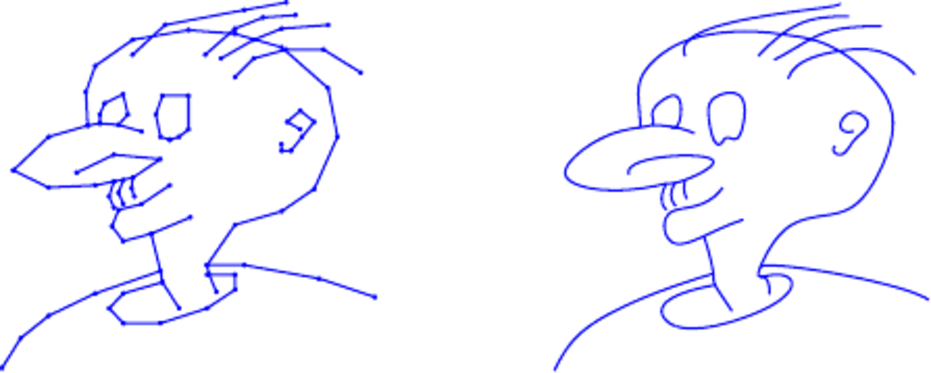
\includegraphics[width=0.7\textwidth]{images/spline} % IN UR THESIS
  \end{center}
  \caption{Gl�ttung durch Splines. Links: Streckenzug mit Hilfe von Geraden zwischen zwei Punkten. Rechts: Streckenzug mit Hilfe von kubischen Polynomen. (Daten aus \cite{c11} von \emph{Gerhard Wanner}).}
  \label{fig:cat}
\end{figure}\\
Was auf den ersten Blick auff�llt: Aufgrund kubischer Parabeln entstehen f�r jedes Intervall $[x_i,x_{i+1}]$ vier unbekannte Koeffizienten $a_i, b_i, c_i$ und $d_i$. Bei $n$ verschiedenen Teilintervallen bedeutet das, dass mit Hilfe von $n$ Gleichungen $4n$ unbekannte Koeffizienten bestimmt werden sollen. Um alle Koeffizienten eindeutig bestimmen zu k�nnen, m�ssen weitere Bedingungen herangezogen werden. Die erste Bedingung ist, dass der ermittelte kubische Spline zweimal stetig differenzierbar sein muss. Dadurch wird ein durchgehender Polynomzug erzwungen. Eine weitere Bedingung ist, dass kubische Splines eine Minimalit�tsbedingung f�r die zweite Ableitung erf�llen m�ssen, was sie gegen�ber anderen Splines besonders interessant macht.\\
\hspace*{0.45cm}Mathematisch formuliert wird nach einer Funktion \mbox{$s:[x_0, x_n] \rightarrow \mathbb R$} mit $x_0 < \dots < x_n$ und folgenden Eigenschaften gesucht:
\begin{itemize}
\item[(a)] $s(x_i) = y_i$ , $i=0,\dots, n$\ ,
\item[(b)] $s \in C^2([x_0,x_n])$\ ,
\item[(c)] $\int_{x_0}^{x_n}(s^{\prime\prime}(x))^2  \partial x \rightarrow min\ ,$
\item[(d)] $s_i(x)=a_i(x-x_i)^3 + b_i(x-x_i)^2 + c_i(x-x_i) + d_i$ mit $x \in [x_i, x_{i+1}]$ und $i=0,\dots,n-1$.
\end{itemize}
Um das Gleichungssystem eindeutig zu l�sen, werden $4n$ Bedingungen ben�tigt. F�r jedes der $n$ Intervalle sind zwei Interpolationsbedingungen zu erf�llen:
\begin{align*}
s_i(x_i) & = y_i\ ,\\
s_i(x_{i+1}) & =y_{i+1}\ .
\end{align*}
Dadurch entstehen $2n$ Bedingungen. Eingesetzt bedeutet das f�r die beiden Endpunkte eines Teilintervalls $[x_i,x_{i+1}]$
\begin{align*}
s_i(x_i) = a_i(x_i-x_i)^3 + b_i(x_i-x_i)^2 + c_i(x_i-x_i) + d_i = d_i &= y_i\ ,\\
s_i(x_{i+1}) = a_i(x_{i+1}-x_i)^3 + b_i(x_{i+1}-x_i)^2 + c_i(x_{i+1}-x_i) + d_i &= y_{i+1}\ .
\end{align*}

Zudem sind alle ($n-2$) inneren St�tzstellen zweimal stetig differenzierbar. Mit den ersten beiden Ableitungen
\begin{align*}
s_i^{\prime}(x) &= 3a_i(x-x_i)^2+2b_i(x-x_i)+c_i\ ,\\
s_i^{\prime\prime}(x) &= 6a_i(x-x_i)+2b_i
\end{align*}
werden weitere $2n-2$ Bedingungen
\begin{align*}
s_i^{\prime}(x_{i+1}) = s_{i+1}^{\prime}(x_{i+1}) \ \ \ \ \ & i = 0,\dots, n-2\ ,\\
s_i^{\prime\prime}(x_{i+1}) = s_{i+1}^{\prime\prime}(x_{i+1}) \ \ \ \ \  & i = 0,\dots, n-2
\end{align*}
erzeugt, die erf�llt werden m�ssen. Die dadurch entstehenden Gleichungen der zweiten Ableitung werden in Abh�ngigkeit von $s^{\prime\prime}$ gel�st:
\begin{align*}
s_i^{\prime\prime}(x_i) &= 6a_i(x_i-x_i)+2b_i = 2b_i\\
\Leftrightarrow \ b_i &= \frac{s_i^{\prime\prime}(x_i)}{2}\\
s_i^{\prime\prime}(x_{i+1}) &= 6a_i(x_{i+1}-x_i)+2b_i = 6a_i(x_{i+1}-x_i) + 2\frac{s_i^{\prime\prime}(x_i)}{2}\\
\Leftrightarrow a_i &= \frac{s_i^{\prime\prime}(x_{i+1})-s_i^{\prime\prime}(x_i)}{6(x_{i+1}-x_i)}
\end{align*}
Diese Gleichungen in $s_i(x_{i+1})$ eingesetzt ergeben:
\begin{align*}
s_i(x_{i+1}) & =y_{i+1} \\
&=a_i(x_{i+1}-x_i)^3+b_i(x_{i+1}-x_i)^2+c_i(x_{i+1}-x_i)+d_i\\
&= \frac{s_i^{\prime\prime}(x_{i+1})-s_i^{\prime\prime}(x_i)}{6}(x_{i+1}-x_i)^2+\frac{s_i^{\prime\prime}(x_i)}{2}(x_{i+1}-x_i)+c_i(x_{i+1}-x_i)+y_i\\
\Leftrightarrow c_i &= \frac{y_{i+1}-y_i}{x_{i+1}-x_i}-\frac{2(x_{i+1}-x_i)s_i^{\prime\prime}(x_i)+(x_{i+1}-x_i)s_{i+1}^{\prime\prime}(x_{i+1})}{6}
\end{align*}
Mit Hilfe der ersten Ableitung werden die folgenden Berechnungen m�glich:
\begin{align*}
s_i^{\prime}(x_i)&=3a_i(x_i-x_i)^2+2b_i(x_i-x_i)+c_i = c_i\\
s_{i-1}^{\prime}&=3a_{i-1}(x_i-x_{i-1})^2+2b_{i-1}(x_i-x_{i-1})+c_{i-1}
\end{align*}
Mit der Vorraussetzung $s_i^{\prime}(x_i)=s_{i-1}^{\prime}(x_i)$ wird f�r die Berechnung der ben�tigten Koeffizienten das folgende Gesamtkonzept erstellt, wobei zur besseren Darstellung $h_i \coloneqq x_{i+1}-x_i$ gilt:
\[
\begin{pmatrix}
  2(h_0 + h_1)  & h_1           & 0           & \cdots  & 0 \\
  0             & h_2           & 2(h_2+h_3)  & h_3     & \vdots\\
  \vdots        &               &             & \ddots  & \\
  0             & \cdots        &             & h_{n-2} & 2(h_{n-2}+h_{n-1})
\end{pmatrix}
\begin{pmatrix}
  s_1\\
  s_2\\
  \vdots\\
  s_{n-1}
\end{pmatrix}
= 6 \cdot
\begin{pmatrix}
  \frac{y_2-y_1}{h_1}-\frac{y_1-y_0}{h_0}\\
  \frac{y_3-y_2}{h_2}-\frac{y_2-y_1}{h_1}\\
  \vdots\\
  \frac{y_n-y_{n-1}}{h_{n-1}}-\frac{y_{n-1}-y_{n-2}}{h_{n-2}}
\end{pmatrix}
\]
% \\
% F�r die letzten beiden fehlenden Bedingungen, den sogenannten Randbedingungen, gibt es verschiedene M�glichkeiten, so z.\,B.
% \begin{itemize}
% \item freier Rand oder nat�rlicher Spline: $s_0^{\prime\prime}(x_0)=0$ und $s_{n-1}^{\prime\prime}(x_n)=0$
% \item eingespannter Rand: $s_0^{\prime}(x_0)=P^{\prime}(x_0)$ und $s_{n-1}(x_n)=P^{\prime}(x_n)$,
% wobei $P^{\prime}(x_0)$ und $P^{\prime}(x_n)$ vorgegeben, normalerweise entweder durch die Ableitung der zu interpolierenden Funktion P oder durch eine Approximation.
% \item periodische Randbedingung: $s_1^{\prime}(x_0)=s_n^{\prime}(x_n)$ und $s_1^{\prime\prime}(x_0)=s_n^{\prime\prime}(x_n)$
% \end{itemize}
% Gesamthaft haben wir $2n+2(n-1)+2=4n$ Bedingungen. Ausreichend um das Gleichungssystem eindeutig l�sen zu k�nnen. ->

Nach diesen Rechenschritten wird das Gesamtergebnis in Form einer Funktion mit den ermittelten $s_i$ angegeben:
\begin{equation}
s(x)= \left\{
\begin{array}{ll}
s_0(x), &x \in [x_0, x_1]\\
s_1(x), &x \in [x_1, x_2]\\
\ \ \ \ \vdots &\\
s_{n-1}(x), &x \in [x_{n-1},x_n]
\end{array}
\right. .
\end{equation}
Da es sich bei der Spline-Interpolation um ein approximatives Verfahren handelt, spielt die Fehlerabsch�tzung eine wichige Rolle.

\subsubsection{Fehlerabsch�tzung f�r kubische Splines}
\label{ch:np-revocation-schema:sec:spline-error}
F�r eine Funktion $f \in C^2([x_0,x_n])$ und einen zugeh�rigen kubischen Spline $s$ bez�glich \mbox{$x_0<\dots<x_n$} und den Werten $y_k = f(x_k)$, $k=1,\dots,n$ mit nat�rlichen Randbedingungen $s_0^{\prime\prime}(x_0)=0$ und $s_{n-1}^{\prime\prime}(x_n)=0$ gilt die folgende Fehlerabsch�tzung:
\begin{align*}
\max_{x_0\leq x\leq x_n} \left| f(x)-s(x) \right| \leq \frac{1}{2} h^2 \max_{x_0\leq x\leq x_n} \left| f''(x)\right|
\end{align*}
mit $h:= \max_{0\leq k<n-1} (x_{k+1}-x_k)$. Der Beweis w�rde �ber den Rahmen der Studienarbeit hinausgehen, kann aber unter \cite{c11} nachgelesen werden.

%% ==============================
\subsection{Kubische Spline-Interpolation im Naor-Pinkas-Verfahren}
\label{ch:np-revocation-schema:sec:spline-np}
%% ==============================
Die Umsetzung der Spline-Interpolation im Naor-Pinkas-Verfahren bringt einige Schwierigkeiten mit sich. Diese werden in diesem Abschnitt n�her erl�utert.

\subsubsection{Wertebereich des Splines}
Auf den ersten Blick f�llt auf, dass die zu ermittelnde Funktion $s(x)$ im Wertebereich $[x_0,x_n]$ beschr�nkt ist. Jedoch wird im Naor-Pinkas-Verfahren der geheime Schl�ssel $\mathcal S$ standardm��ig im Punkt $x=0$ gespeichert. Um  $0 \in [x_0,x_n]$ sicherzustellen, muss mindestens ein St�tzwert $x_{neg} < 0$ existieren. Dies kann ein vom Gruppencontroller ausgew�hlter Dummy-Benutzer $u_d \in \mathcal R$ sein. Sollte es sich nicht um einen Dummy handeln, muss zu jeder Zeit sichergestellt werden, dass mindestens ein Wertepaar $<I_{u_i},P(I_{u_i})>$ eines Empf�ngers $u_i \in \mathcal R$ existiert. Grund hierf�r ist, dass ein Empf�nger $u \in \mathcal N \setminus \mathcal R$ nicht in der Menge $\mathcal R$ der �bertragenen Nachricht vorkommt. Anders ausgedr�ckt kann in solch einer Konstellation lediglich der Empf�nger $u_i$ mit $I_{u_i}<0$ den Schl�ssel $\mathcal S$ berechnen, da au�er ihm niemand eine Funktion $s(x)$ interpolieren kann, welche im Wertebereich $x<0$ liegt. Diese Situation wird nochmal in der folgenden Abbildung \ref{fig:bereich} dargestellt.

\begin{figure}[ht]
  \begin{center}
    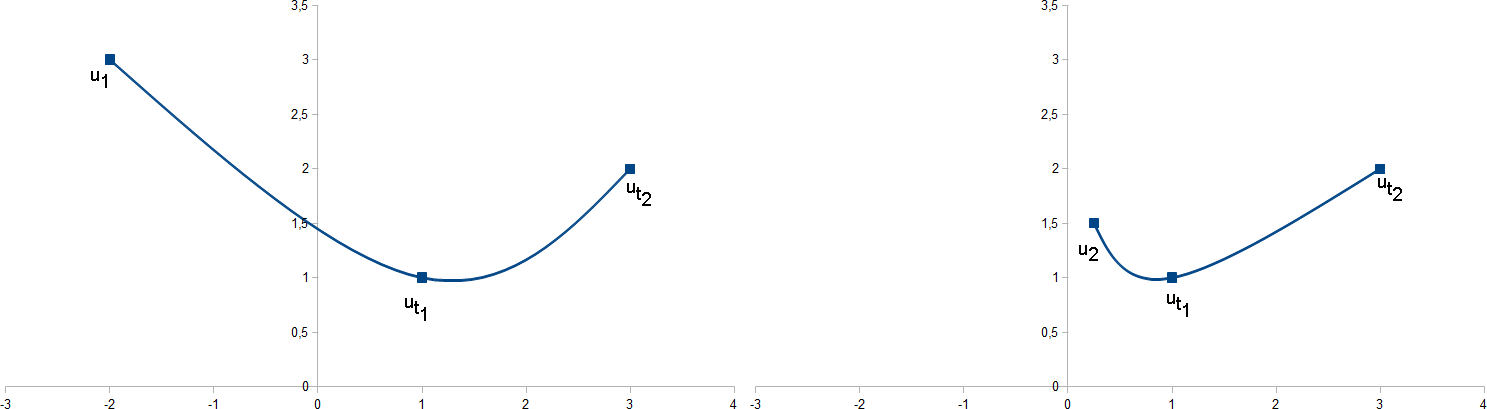
\includegraphics[width=1\textwidth]{images/Bereich} % IN UR THESIS
  \end{center}
  \caption{Wertebereich der Spline-Interpolation. Links aus der Sicht des Empf�ngers $u_1$ mit $I_{u_1}<0$, rechts aus der Sicht des Empf�ngers $u_2$}
  \label{fig:bereich}
\end{figure}

\subsubsection{Wert des Schl�ssels}
Eine weitere Untersuchung der Spline-Interpolation ergibt einen wichtigen Grund, weshalb diese im Naor-Pinkas-Verfahren nicht angewendet werden kann.
Hierzu soll die in Abbildung \ref{fig:schluessel} definierte Situation mit den Teilnehmern $I_{u_1}, I_{u_2} \in \mathcal N \setminus \mathcal R$ und $I_{u_1}, I_{u_2} < 0$ genauer betrachtet werden. Seien $I_{u_{t_1}}, I_{u_{t_2}} \in \mathcal R$ mit der Sortierung $I_{u_1} < I_{u_2} < 0 < I_{u_{t_1}} < I_{u_{t_2}}$ gegeben. Ferner seien den Empf�ngern $u_1$ und $u_2$ die Werte $s^{\prime}(I_{u_{t_i}})$ und $s^{\prime\prime}(I_{u_{t_i}})$ mit $i=1,2$ bekannt.\\

\begin{figure}[h]
  \begin{center}
    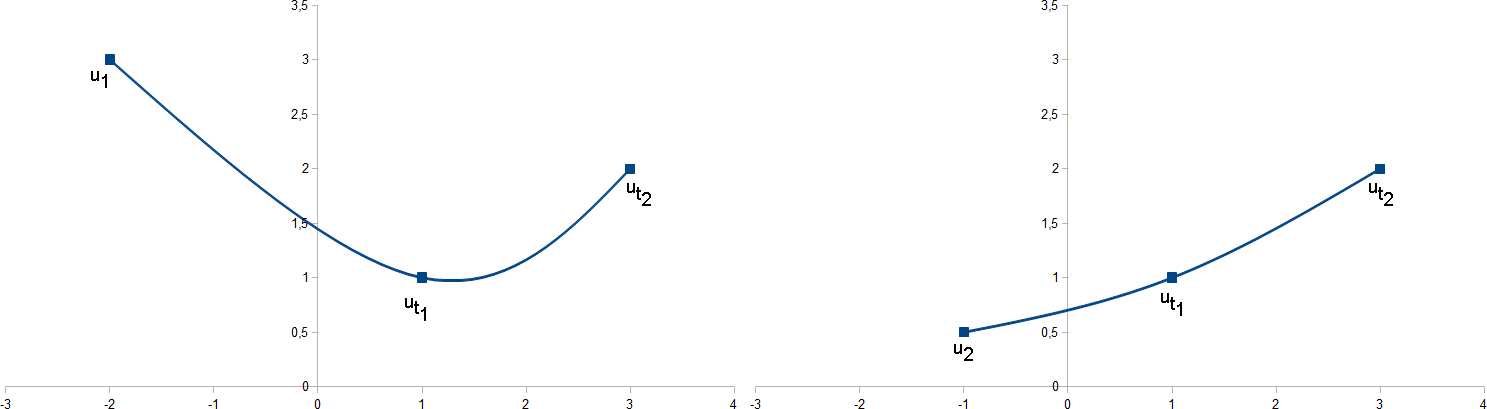
\includegraphics[width=1\textwidth]{images/Punkt0} % IN UR THESIS
  \end{center}
  \caption{Wert des Schl�ssels. Links aus der Sicht des Empf�ngers $u_1$, rechts aus der Sicht des Empf�ngers $u_2$}
  \label{fig:schluessel}
\end{figure}

Wie hier bereits mit einigen Beispielwerten gezeigt wird, ist der Schl�ssel im Punkt $x=0$ aus der jeweiligen Sicht der Empf�nger $u_1$ und $u_2$ nicht eindeutig. Dies soll nochmals betonen, dass die Spline-Interpolation nicht ohne weiteres im Naor-Pinkas-Verfahren angewendet werden kann.


% Da der mathematische Beweis �ber den Rahmen dieser Studienarbeit hinausgehen w�rde, wodurch in dieser Situation die Sicherheit des Verfahrens nicht mehr gew�hrleistet werden k�nnte.

%% ==============================
\subsection{Fazit}
\label{ch:np-revocation-schema:sec:spline-fazit}
%% ==============================
Die Spline-Interpolation generiert abschnittsweise glatte und stetig differenzierbare Funktionen und vermeidet starke Oszillationen im Funktionsverlauf. Jedoch kann sie nicht ohne weiteres im Naor-Pinkas-Schema angewendet werden, da es sich bei dieser Interpolation um ein approximatives Verfahren handelt.\\
\hspace*{0.45cm}Zum einen liegt es am definierten Wertebereich der Funktion, zum anderen am ermittelten Wert des Schl�ssels. Ersteres k�nnte noch einfach durch einen Dummy-Benutzer oder durch Festlegung des Schl�ssels an einer anderen Stelle behoben werden. Das zweite Problem ist nicht ohne weiteres offensichtlich l�sbar. Durch die Verwendung eines h�heren Polynomgrades k�nnte der ermittelte Wert n�her am tats�chlichen liegen, jedoch erh�ht sich dadurch gleichzeitig der Berechnungsaufwand. Eine weitere M�glichkeit w�re, einen Schwellenwert f�r den Wert des Schl�ssels zu benutzen. Jedoch w�rde sich die Sicherheit des Schemas in diesem Fall reduzieren, da der Schl�ssel nicht mehr eindeutig berechnet werden, sondern sich lediglich im Schwellenwertbereich des Schl�ssels befinden m�sste.

\newpage

%% ==============================
\section{Vergleich der Interpolationsm�glichkeiten}
\label{ch:np-revocation-schema:sec:fazit-all}
%% ==============================

Wie bisher gezeigt wurde, k�nnen im Naor-Pinkas-Schema die Lagrange-Interpolation und die Newton-Interpolation gleicherma�en angewendet werden. In diesem Abschnitt sollen diese miteinander verglichen werden.\\
\hspace*{0.45cm}Diesbez�glich werden die Anzahl der verschiedenen Operationen (Addition A, Multiplikation M, Division D und Exponentiation E) der Lagrange- und Newton-Interpolation im Naor-Pinkas-Schema genauer untersucht.

\subsection{Additionen}
\label{sub:addition}
Die im Abschnitt \ref{ch:np-revocation-schema:sec:Aufwand} ermittelte Gesamtanzahl an Addition in der Lagrange-Interpolation im Naor-Pinkas-Schema betr�gt nach \eqref{eq:la_formel_gesamt}:
\[
  Anzahl_{L_A} = t\cdot(t+1)\,A
\]
Im Abschnitt \ref{ch:np-revocation-schema:sec:newton-overflow} wurde f�r die Newton-Interpolation folgende Anzahl an Additionen ermittelt:
\[
  Anzahl_{N_L} = \sum_{i=1}^t 2^{i-1}\cdot i\,A% = \frac{t(t+1)(2t+1)}{6}\,A
\]
Die folgende Tabelle zeigt sehr deutlich, wie sehr sich diese zwei Werte in Abh�ngigkeit von der Anzahl an unerlaubten Empf�ngern auswirkt:
\begin{center}
\begin{tabular}{c|c|c}
$|\mathcal R|$ & $Anzahl_{L_A}$ & $Anzahl_{N_A}$\\
\hline
10 & 110 & 9217\\
25 & 650 & 805306369\\
50 & 2550 & $5,517\cdot 10^{16}$\\
\end{tabular}
\end{center}
Die Anzahl an Additionen steigt in der Newton-Interpolation im Naor-Pinkas-Schema rasant an.

\subsection{Multiplikationen}
\label{sub:multiplikationen}
Aus \eqref{eq:la_formel_gesamt} ermitteln wird die Anzahl an Multiplikationen f�r die Lagrange-Interpolation im Naor-Pinkas-Schema:
\[
  Anzahl_{L_M} = \left(2\cdot(t^2-1)+t\right)\,M
\]
Im Vergleich dazu die aus der Newton-Interpolation:
\[
  Anzahl_{N_M} = \sum_{i=1}^t 2^{i-1}\cdot (i-1)\,M+i\,M
\]
Auch hier ist das Ziel nun, diese zwei Ergebnisse miteinander in Beziehung zu setzen:
\begin{center}
\begin{tabular}{c|c|c}
$|\mathcal R|$ & $Anzahl_{L_M}$ & $Anzahl_{N_M}$\\
\hline
10 & 208 & 8249\\
25 & 1273 & 771752263\\
50 & 5048 & $5,404\cdot 10^{16}$\\
\end{tabular}
\end{center}
�hnlich wie bei der Anzahl an Additionen steigt die Anzahl an Multiplikationen bei der Newton-Interpolation schneller an.

\subsection{Divisionen}
\label{sub:divisionen}
Entsprechend \eqref{eq:la_formel_gesamt} werden bei der Lagrange-Interpolation
\[
  Anzahl_{L_D} = (t+1)\,D
\]
Divisionen bei einem einzelnen Empf�nger ben�tigt, um das Polynom an der Stelle $g^{rP(0)}$ ermitteln zu k�nnen. Im Vergleich dazu werden
\begin{align*}
  Anzahl_{N_D} &= \sum_{i=1}^t \left( 2^i-1+2^{i-1} \right)\,D
  % \\
  % &=\left(\sum_{i=1}^t 2^i - \sum_{i=1}^t 1 + \sum_{i=1}^t i\right) \ D\\
  % &= (2^{t+1}-2) - t + \frac{t(t+1)}{2}\ D
\end{align*}
Anzahl an Divisionen bei der Newton-Interpolation gebraucht. Auch hier soll durch ein paar Werte gezeigt werden, dass diese Anzahl an beider Interpolationen sich stark voneinander unterscheiden:
\begin{center}
\begin{tabular}{c|c|c}
$|\mathcal R|$ & $Anzahl_{L_D}$ & $Anzahl_{N_D}$\\
\hline
10 & 11 & 3059\\
25 & 26 & 100663268\\
50 & 51 & $3,378\cdot10^{15}$\\
\end{tabular}
\end{center}

\subsection{Exponenten-Berechnungen}
\label{sub:exponentiation}
Bei der Lagrange-Interpolation werden
\[
  Anzahl_{L_E} = (t+2)\,E
\]
Exponenten-Berechnungen bei einem einzelnen Empf�nger ben�tigt, um das Polynom an der Stelle $g^{rP(0)}$ ermitteln zu k�nnen. Bei der Newton-Interpolation im Naor-Pinkas-Schema werden im Vergleich dazu
\begin{align*}
  Anzahl_{N_E} = (t+2 + \sum_{i=1}^t 2^{i-1})\,E
\end{align*}
Anzahl an Exponenten-Berechnungen bei der Newton-Interpolation gebraucht. Es ist leicht zu zeigen, dass $Anzahl_{L_E} < Anzahl_{N_E}$ gilt. Jedoch sollen auch hier ein paar Beispielwerten aufzeigen, wie schnell ein gro�er Unterschied beider Interpolationen entsteht:
\begin{center}
\begin{tabular}{c|c|c}
$|\mathcal R|$ & $Anzahl_{L_E}$ & $Anzahl_{N_E}$\\
\hline
10 & 12 & 1035\\
25 & 27 & 33554458\\
50 & 52 & $1,126\cdot10^{15}$\\
\end{tabular}
\end{center}

\subsection{Fazit}
\label{sub:fazit}
In den vorherigen Abschnitten wurde gezeigt, dass durch die notwendigen Umformungen in der Newton-Interpolation im Naor-Pinkas-Schema gegen�ber der Lagrange-Interpolation mehr Berechnungsschritte ben�tigt. Die Newton-Interpolation ist daher nicht besser geeignet. Die hier ermittelten Werte bei relativ kleinem $|\mathcal R|$ best�tigen dies. Der Unterschied spielt vor allem bei zustandslosen Empf�ngern mit beschr�nkter Speicherm�glichkeit eine gro�e Rolle und sollte nicht zu vernachl�ssigen sein.

% subsection fazit (end)

% \newpage
% Dabei wird besonders auf die arithmetischen Flie�kommaoperationen pro Sekunde ($FLOPS$ = Floating-point Operations per Second) eingegangen, wobei die �bliche Gewichtungen der Operationen in der folgenden Tabelle festgehalten werden:
% \begin{center}
% \begin{tabular}{l|l}
% \textbf{Gleitpunktoperation} & \textbf{Gewichtung} \\
% \hline
% Addition, Subtraktion, Multiplikation & 1 FLOPS\\
% Division & 4 FLOPS\\
% Exponentialfunktion & 8 FLOPS
% \end{tabular}
% \end{center}
% Werden die ermittelten Werte f�r die Lagrange-Interpolation aus \eqref{eq:la_formel_gesamt} genauer betrachtet, ergibt das
% \begin{align*}
% &\ \ \ \ \, (t^2+2t)\,M + t\cdot (t+1)\,D + t\cdot(t+1)\,A + (t+2)\,E\\
% &= (t^2+2t) + 4t\cdot (t+1) + t\cdot(t+1) + 8(t+2)\\
% &= 6t^2 + 15t + 16
% \end{align*}
% und aufgrund von \eqref{eq:newton-aufwand-gesamt} erh�lt die Newton-Interpolation die Gesamtgewichtung
% \begin{align*}
% &\ \ \ \ \left( \frac{t\cdot (t+1)}{2} \right)\,M + \left( \frac{t\cdot(t+1)}{2} \right)\,D + t\cdot(t+1)\,A+(t+1)\,E\\
% &= \frac{t\cdot (t+1)}{2} + 4\cdot \left( \frac{t\cdot(t+1)}{2} \right) + t\cdot(t+1) + 8(t+1)\\
% &= 3,5t^2 + 11,5t + 8\ .
% \end{align*}
% Das Ziel ist nun, diese zwei Ergebnisse zueinander in Beziehung zu setzen. Dabei wird mit einer Anzahl an unerlaubten Empf�ngern von $t>0$ folgende Absch�tzung gemacht:
% \[
%   6t^2 + 15t + 16 > 6t^2 + 15t + 8 > 6t^2 + 11,5t + 8 > 3,5 t^2 + 11,5t + 8
% \]
% Zusammengefasst bedeutet dieses Ergebnis, dass die Anzahl an notwendigen Operationen eines Empf�ngers bei der Newton-Interpolation im Vergleich zur Lagrange-Interpolation f�r jede beliebige Anzahl an unerlaubten Empf�ngern geringer ausf�llt. Dadurch kann das Naor-Pinkas-Verfahren mit Hilfe der Newton-Interpolation effizienter ausgef�hrt werden.

% Dass dieses Ergebnis eine nicht zu vernachl�ssigende Bedeutung hat, soll die folgende Tabelle darstellen.
% \begin{center}
% \begin{tabular}{c|c|c}
% \textbf{Unerlaubte Empf�nger $t$} & \textbf{Gesamtgewichtung Lagrange} & \textbf{Gesamtgewichtung Newton} \\
% \hline
% 100 & 61516 & 36158\\
% 1000 & 6015016 & 3511508\\
% 10000 & 600150016 & 350115008\\
% \end{tabular}
% \end{center}
% Ab einer gewissen Anzahl an unerlaubten Empf�ngern und mit Hilfe der oben definierten �blichen Gewichtung der Operationen w�chst der Unterschied der Anzahl an $FLOPS$ zwischen der Lagrange- und der Newton-Interpolation auf das $\frac{6}{3,5}$-fache an.

\newpage

%% Encoding: ISO8859-1 %%

\chapter{Asmuth-Bloom-Verfahren}
\label{ch:ab}
%% ==============================

In diesem Abschnitt wird ein kurzer Einblick in das Asmuth-Bloom-Verfahren \cite{ab83} gegeben, welches den aus der Zahlentheorie bekannten chinesischen Restsatz anwendet. Hierzu werden jedoch einige Vorkenntnisse ben�tigt.

\section{Simultane Kongruenzen ganzer Zahlen}
\label{ch:ab:sec:cr:sub:sim_kon}

Eine simultane Kongruenz ganzer Zahlen ist ein System von linearen Kongruenzen
\[
\begin{matrix}
x & \equiv & a_1 & \pmod{m_1} \\
x & \equiv & a_2 & \pmod{m_2} \\
  & \vdots &     &            \\
x & \equiv & a_n & \pmod{m_n}, \\
\end{matrix}
\]
wof�r der unbekannte Wert $x$ f�r alle Kongruenzen bestimmt werden soll, falls solch ein Wert �berhaupt existiert. Wenn eine L�sung $x$ existiert, dann sind $\mathcal M \coloneqq kgV(m_1,\dots,m_n)$ und die Zahlen $x+k\mathcal M$ mit $k\in \mathbb Z$ alle L�sungen dieses Systems.

\section{Chinesischer Restsatz}
\label{ch:ab:sec:cr}

Mit Hilfe des chinesischen Restsatzes kann unter gewissen Einschr�nkungen eine Aussage �ber simultane Kongruenzen getroffen werden. Dabei seien $m_1,\dots,m_n$ paarweise teilerfremde, nat�rliche Zahlen. Dann existiert f�r beliebige Zahlen $a_1,\dots,a_n \in \mathbb Z$ eine Zahl $x$, die das folgende System von linearen Kongruenzen mit $i = 1, \dots, n$ erf�llt:
\[
x \equiv a_i \pmod{m_i}
\]
Alle L�sungen sind kongruent modulo $\mathcal M \coloneqq m_1m_2\cdots m_n$.

Sei $\mathcal M_i=\mathcal M \setminus m_i$. Das Finden einer L�sung erfolgt mit dem erweiterten euklidischen Algorithmus, wobei zwei Zahlen $r_i$ und $s_i$ berechnet werden, sodass die Gleichung
\[
r_i \cdot m_i + s_i \cdot \mathcal M_i = 1
\]
stimmt. Ferner gilt durch $e_i \coloneqq s_i\cdot M_i$
\[
e_i \equiv 1 \pmod{m_i}
\]
\[
e_i \equiv 0 \pmod{m_j}
\]
f�r $j \neq i$. Die L�sung der simultanen Kongruenz ist definiert durch:
\begin{align}
x \coloneqq \sum_{i=1}^n a_i e_i \ .
\end{align}

\section{Asmuth-Bloom-Secret-Sharing-Schema}
\label{sec:ashmuth_bloom_secret_sharing_scheme}

Im Asmuth-Bloom-Secret-Sharing-Schema werden zwei Phasen ben�tigt, um das Geheimnis verteilen und rekonstruieren zu k�nnen.
\begin{itemize}
  \item
  \textbf{Initialisierungsphase}\\
  In dieser Phase w�hlt der Gruppencontroller eine Menge von paarweisen teilerfremden Zahlen $m_0 < m_1 < \dots < m_n$, sodass folgende Ungleichung gilt:
  \begin{align}
    \label{ab-bedingung}
    \prod_ {i=1}^t m_i > m_o \prod_{i=1}^{t-1} m_{n-i+1}
  \end{align}
  Ferner werden $\mathcal M \coloneqq \prod_{i=1}^{t}m_i$ und das Geheimnis $\mathcal S$ definiert. Letzteres wird so gew�hlt, dass $m_0 > \mathcal S$ gilt. Im n�chsten Schritt berechnet der Gruppencontroller
  \[
    y=\mathcal S + Am_0\ ,
  \]
  wobei $A$ eine positive, zuf�llig ausgew�hlte Zahl ist, sodass die Bedingung $0 \leq y < \mathcal M$ erf�llt wird. Im letzten Schritt sendet der Gruppencontroller jedem Empf�nger $i$ das ihm zugewiesenen Share
  \[
    y_i = y \mod{m_i}\,.
  \]
  \item
  \textbf{Kombinierungsphase}\\
  Gegeben sei ein Zusammenschluss $\mathcal N'$ von $t < n$ Empf�ngern, welche das Geheimnis in dieser Phase rekonstruieren sollen. Ferner sei noch $M_{\mathcal N'} \coloneqq \prod_{i\in \mathcal N'}m_i$ und das System von Kongruenzen
  \[
    y \equiv y_i \pmod{m_i}
  \]
  f�r $i\in \mathcal N'$ gegeben. Mit Hilfe des chinesischen Restsatzes wird der Wert $y$ aus $\mathbb Z_{\mathcal M_{\mathcal N'}}$ eindeutig bestimmt. Das Geheimnis $\mathcal S$ kann im letzten Schritt wie folgt ermittelt werden:
  \[
    \mathcal S = y \mod{m_0}\,.
  \]
  Diese L�sung ist wegen der Bedingung $y<\mathcal M \leq \mathcal M_{\mathcal N'}$ in $\mathbb Z_{\mathcal M}$ eindeutig.
\end{itemize}

Das Schema ist sicher, solange eine Vereinigung von maximal $t-1$ unerlaubten Empf�ngern sichergestellt wird. Eine detaillierte Analyse der Sicherheit kann in der ver�ffentlichten Arbeit von Quisquater et al. \cite{qpv02} nachgelesen werden. In dieser wird unter anderem das Asmuth-Bloom- und weitere Secret-Sharing-Schemas basierend auf dem chinesischen Restsatz analysiert.
\newpage

\section{Ausblick: Anwendung als Revocation-Schema}

Die Anwendung Asmuth-Bloom-Verfahrens als Revocation-Schema analog zum Noar-Pinkas-Schema bringt eine Problematik mit sich. Der f�r die Berechnung notwendige Wert $y_i$ des Empf�ngers $i$ kann lediglich vom Gruppencontroller bestimmt werden, da nur ihm der Session-Schl�ssel $y = \mathcal S + Am_0$ bekannt ist. Im Umkehrschluss bedeutet das, dass der Gruppencontroller vor der �bertragung der Nachricht jedem erlaubten Empf�nger seinen Share, beispielsweise �ber einen privaten Kanal, mitteilen m�sste.\\
\hspace*{0.45cm}Beim Naor-Pinkas-Schema kann jeder erlaubte Empf�nger $i$ anhand der �bermittlung von $g^r$ und der gespeicherten Information $P(I_i)$ den erforderlichen ($t+1$)-ten Wert $g^{rP(I_i)}$ f�r die eindeutige Bestimmung des Polynoms ermitteln. Dies ist im Asmuth-Bloom-Verfahren nicht m�glich, da der Wert $y_i$ direkt �ber den Session-Schl�ssel mit Hilfe einer Modulo-Operation berechnet wird.\\
\\
Kann jedoch das Naor-Pinkas-Schema im Asmuth-Bloom-Verfahren angewendet werden, falls jeder erlaubter Empf�nger $i$ seinen pers�nlichen Share $y_i$ kennt?\\
\hspace*{0.45cm}Angenommen das Geheimnis $\mathcal S$ wird mit Hilfe eines Generators $g$ und einem beliebigen und zuf�lligen Wert $r$ in den Expontenten verlagert, sodass der neue Schl�ssel durch $g^{rS}$ definiert wird. Zudem existieren paarweise, teilerfremde Zahlen $m_0 < m_1 < \dots < m_n$, wobei $m_0 > \mathcal S$ gilt. Aufgrund der letzt genannten Bedingung k�nnte durch das Verlagern des Schl�ssels in den Exponenten das Finden der Werte $m_1, \dots, m_n$ aufwendiger werden als geplant, da bereits der Startwert $m_0$ gro� sein kann. Ferner berechnet der Gruppencontroller $y=\mathcal S + Am_0$. Zuz�glich seien die Ungleichung aus \ref{ab-bedingung} und die Bedingung $0 \leq y < \mathcal M$ erf�llt. Das gew�nschte Ziel ist, die gleiche �bertragung wie beim Naor-Pinkas-Schema zu erreichen:
\begin{align*}
<g^r, g^{r\,y_{u_1}}, g^{r\,y_{u_2}}, \dots ,g^{r\,y_{u_t}}, m_{u_1},  m_{u_2}, \dots,  m_{u_t} >.
\end{align*}
% Dies ist jedoch Aufgrund der Modulo-Eigenschaft nicht ohne weiteres m�glich.
Hierzu wird die Berechnung eines einzelnen Shares $y_i$ genauer betrachtet:
\begin{align*}
  y_i = y \mod m_i
\end{align*}
Um den eindeutigen Wert $y$ bestimmen zu k�nnen, wird ein Kongruenzsystem von $t$ Kongruenzen ben�tigt:
\begin{align*}
  y \equiv y_i \pmod{m_i}\,.
\end{align*}
Einem Empf�nger wird bei der �bertragenen Nachricht jedoch nur die in den Exponenten verlagerten Shares �bermittelt. Dieser m�sste folglich folgende Berechnung
\begin{align*}
  y \equiv g^{r\,y_i} \pmod{m_i}
\end{align*}
durchf�hren. Dies f�hrt jedoch nicht zum gew�nschten Ergebnis. Anders ausgedr�ckt ben�tigt jeder Empf�nger die f�r die Berechnung notwendigen Shares der anderen Empf�nger in Klartext. Es wurde im Rahmen der Studienarbeit kein Weg gefunden, das Asmuth-Bloom-Verfahren als Revocation-Schema basierend auf dem Prinzip von Naor und Pinkas aufzubauen.

\newpage
\section{Fazit}
Im Rahmen dieser Studienarbeit wurde kein Weg gefunden, dass Asmuth-Bloom-Verfahren als Revocation-Schema einzusetzen. Zum einen liegt das an den Shares, welche nur beim Gruppencontroller berechnet und �bermittelt werden k�nnen. Die Unkenntnis des pers�nlichen Geheimnisses k�nnte durch Hinzunahme eines weiteren Kommunikationsweges mit dem Empf�nger gel�st werden. Zum anderen f�hren die notwendigen Bedingungen dazu, dass der Aufwand f�r die Suche nach geeigneten, paarweisen teilerfremden Zahlen, durch das Verlagern des Schl�ssels in den Exponenten, steigen.\\
\hspace*{0.45cm}Das Ziel im Revocation-Schema von Naor und Pinkas hatte den Ursprung, dass der Schl�ssel in ihrem Single-Revocation-Schema nach einmaliger Berechnung bestimmt werden konnte. Aufgrund dieser Situation wurde der Schl�ssel und die notwendigen Shares $P(I_i)$ in den Exponenten verlagert. Anhand der mathematischen Eigenschaft der Lagrange-Interolation konnte dies geschickt ausgenutzt werden. Dies ist im Asmuth-Bloom-Verfahren nicht n�tig, da der Session-Schl�ssel bereits durch das Addieren von $Am_0$ geheim gehalten wird.\\
\hspace*{0.45cm}Ein weiterer Nachteil des Verfahrens wird beim Finden von paarweise teilerfremde Zahlen bemerkbar, wenn die Anzahl an Teilnehmern gro� ist. Die im Abschnitt \ref{sec:ashmuth_bloom_secret_sharing_scheme} definierten Bedingungen m�ssen zu jederzeit erf�llt werden. Beim Naor-Pinkas-Verfahren muss der Gruppencontroller lediglich eine Bedingung erf�llen: Eine St�tzstelle darf nicht an zwei verschiedenen Teilnehmer vergeben werden. Hierbei fallen bis auf die Suche, ob die St�tzstelle bereits vergeben wurde, keine weiteren Kosten an.\\
\hspace*{0.45cm}Trotzdem stellt das Asmuth-Bloom-Verfahren eine interessante Grundlage f�r ein praktisches Secret Sharing dar. In der ver�ffentlichten Arbeit von Kaya und Sel\c{c}uk \cite{ks07} k�nnen weitere interessante Methoden zum Asmuth-Bloom-Verfahren nachgelesen werden. Unter anderem wird in der Arbeit die Verteilung der Shares mit Hilfe der RSA-Funktion im Asmuth-Bloom-Verfahrens n�her untersucht.

%\include{kapitel/05_ergebnisse}
%% Encoding: ISO8859-1 %%

\chapter{Zusammenfassung und Ausblick}
\label{ch:Zusammenfassung}
% (Keine Untergliederung mehr!)
%% ==============================

In dieser Studienarbeit wurden die Grundlagen des Shamir's Secret Sharing-Verfahrens und das darauf basierende Naor-Pinkas-Revocation-Schema genauer erl�utert. Zudem wurde nach alternativen Interpolationsverfahren gesucht, die im Schema angewendet und effizienter ausgef�hrt werden konnten. Die zur Lagrange- sehr �hnliche Newton-Interpolation konnte ohne weitere Probleme in das Schema eingebaut werden, wobei der notwendige Schl�sselberechnungsaufwand eines Empf�ngers zu jedem Zeitpunkt geringer ausf�llt als bei der etwas langsameren Interpolation mit Hilfe der Lagrange-Basisfunktionen.\\
\hspace*{0.45cm}Die approximative Interpolation mit Splines f�hrte zum Ergebnis, dass diese nicht ohne weiteres als Interpolationsm�glichkeit im Naor-Pinkas-Revocation-Schema angewendet werden kann. Bei der Umsetzung entstanden zwei Probleme. Das erste war die Sicherstellung von $x=0 \in [x_0,x_n]$, was relativ einfach behoben werden konnte, indem ein Dummy-Benutzer $x_d < 0$ hinzugef�gt wurde. Eine weitere L�sung ist die Verwendung eines anderen Schl�ssels $\mathcal S \in [x_0,x_n]$. Das zweite Problem kann jedoch nicht ohne weiteres behoben werden. Es handelt sich hierbei um die Nichteindeutigkeit des berechneten Wertes f�r den Schl�ssel $\mathcal S$. Als L�sungsvorschlag wurden eine Schwellenwertfunktion und Polynome von h�herem Grad in den Intervallabschnitten beschrieben, welche jedoch die Effizienz und die Sicherheit des Revocations-Schemas reduzieren w�rden.\\
\hspace*{0.45cm}Im darauf folgenden Kapitel wurde das Asmuth-Bloom-Secret-Sharing-Schema genauer beschrieben. Das Ziel war, das Naor-Pinkas-Revocation-Schema so einzubauen, dass es als effizientes Broadcasting-Schema angewendet werden kann. In der Analyse fiel auf, dass dies nicht ohne weiteres m�glich ist. Grund hierf�r sind die vom Gruppencontroller berechneten Shares des Session-Schl�ssels. Diese k�nnen nicht von einem Empf�nger selber berechnet oder hergeleitet werden. Zu einem weiteren Problem f�hrte die Modulo-Eigenschaft. Diese f�hrte aufgrund der Verlagung der Shares in den Exponenten nicht zum gew�nschten Ergebnis. Weitere Untersuchungen zu diesem Bereich k�nnen in der vorgestellten Arbeit von Kaya und Sel\c{c}uk \cite{ks07} nachgelesen werden.\\
\hspace*{0.45cm}Es existieren weitere Secret-Sharing-Verfahren, welche au�erhalb des Bereichs der Zahlentheorie und der Interpolationen liegen. Darunter f�llt auch die von Blakley \cite{b79} ver�ffentlichte Arbeit. In diesem Schema werden in einem $n$-dimensionalen Raum $n$ nichtparallele Hyperebenen definiert. Dadurch wird ein eindeutiger Schnittpunkt im Raum generiert, welcher jedoch nur mit Hilfe der $n$ Hyperebenen eindeutig ermittelt werden kann. Auch hier stellt sich die Frage, ob mit Hilfe des Naor-Pinkas-Revocation-Schemas die notwendigen Informationen in den Exponenten gezogen werden k�nnen, um auf diese Art und Weise ein effizientes Revocation-Schema zu erstellen.\\
\hspace*{0.45cm}Aufgrund der mathematischen Eigenschaften bieten Secret-Sharing-Verfahren eine gute und effiziente M�glichkeit, den Schl�ssel vor unerlaubten Empf�ngern geheim zu halten. Mit ver�ffentlichten Arbeiten wie beispielsweise der von Naor und Pinkas werden solche Schemata weiter verbessert und optimiert, um in der heutigen digitalen Welt mehr Sicherheit gew�hleisten zu k�nnen.

%% ++++++++++++++++++++++++++++++++++++++++++
%% Anhang
%% ++++++++++++++++++++++++++++++++++++++++++

\appendix
%\include{anhang_a}
%\include{anhang_b}

%% ++++++++++++++++++++++++++++++++++++++++++
%% Literatur
%% ++++++++++++++++++++++++++++++++++++++++++
%  mit dem Befehl \nocite werden auch nicht
%  zitierte Referenzen abgedruckt
\cleardoublepage
\phantomsection
\addcontentsline{toc}{chapter}{\bibname}
%%
%\nocite{*} % nur angeben, wenn auch nicht im Text zitierte Quellen
%           % erscheinen sollen
\bibliographystyle{geralpha} % abbrvnat unsrtnat
% spezielle Zitierstile: Labels mit vier Buchstaben und Jahreszahl
\bibliography{ausarbeitung}
%% ++++++++++++++++++++++++++++++++++++++++++
%% Index
%% ++++++++++++++++++++++++++++++++++++++++++
\ifnotdraft{
\cleardoublepage
\phantomsection
\printindex            % Index, Stichwortverzeichnis
}
\end{document}

